\documentclass[final,a4paper,openany,12pt]{mwbk}
%\documentclass[final,a4paper,openright,12pt]{mwbk} % każdy rozdział zaczyna się na stronie nieparzystej
\usepackage{polski}
\usepackage[utf8]{inputenc}
\usepackage{fancyhdr}
\usepackage{url}
\usepackage{algorithm}
\usepackage{algpseudocode}
\usepackage{enumerate}
\usepackage{subcaption}
\captionsetup{compatibility=false}
\usepackage{titlesec}
\usepackage{amsmath}

\titleformat{\section}[runin]
{\normalfont\Large\bfseries}{\thesection}{1em}{}
\titleformat{\subsection}[runin]
{\normalfont\large\bfseries}{\thesubsection}{1em}{}



\usepackage{makeidx}  % allows index generation
\usepackage{graphicx} % standard LaTeX graphics tool
                      % for including eps-figure files
\graphicspath{{img/}}
\usepackage{float}

\prefixing %polskie znaki: /a /c /e /z /x /o /s /l /A /C itd.

\renewcommand*\listalgorithmname{Spis algorytmów\protect} % łatka na niedoróbkę w spisie algorytmów - nie usuwać!

% zestaw przydatny, kiedy trzeba regulować szerokość kolumn w tablicy:
%%\usepackage{longtable}
%\usepackage{array}
%\newcolumntype{L}[1]{>{\raggedright\let\newline\\\arraybackslash\hspace{0pt}}m{#1}}
%\newcolumntype{C}[1]{>{\centering\let\newline\\\arraybackslash\hspace{0pt}}m{#1}}
%\newcolumntype{R}[1]{>{\raggedleft\let\newline\\\arraybackslash\hspace{0pt}}m{#1}}

\newtheorem{twr}{Twierdzenie}[section]

% ustawienia do wydruku dwustronnego z uwzględnieniem dodatkowego miejsca na zszycie
\setlength{\oddsidemargin}{0.46cm}   %margines nieparzysty
\setlength{\evensidemargin}{-0.54cm} %margines parzysty
\setlength{\textwidth}{16cm}         %szerokość tekstu na stronie
\linespread{1.1}    % lekkie zwiększenie odstępu między liniami, żeby tekst nie był taki ścisły, ponieważ
                    % Odstęp pojedynczej interlinii nie jest komfortowy, kiedy trzeba czytać strony A4
% koniec ustawień

%\makeindex            % used for the subject index
                      % please use the style sprmidx.sty with
                      % your makeindex program
\begin{document}

\begin{titlepage}
\vspace{-0.5cm}

{\centering
{\footnotesize
\begin{tabular}{c}
UNIWERSYTET KARDYNAŁA STEFANA WYSZYŃSKIEGO\\
W WARSZAWIE\\
\end{tabular}
}
\vspace{2.5cm}

{\footnotesize
\begin{tabular}{c}
WYDZIAŁ MATEMATYCZNO-PRZYRODNICZY\\
SZKOŁA NAUK ŚCISŁYCH\\
\end{tabular}
}
\vspace{2.5cm}

\renewcommand{\arraystretch}{1.5} % zwiększamy odległość między wierszami

{\normalsize
\begin{tabular}{c}
Katarzyna Mitrus\\
Michał Słotwiński\\
\end{tabular}
}

\vspace{1.5cm}

{\large
\begin{tabular}{c}

Wprowadzenie do Przetwarzania Obrazów\\
Sprawozdanie z laboratorium\\

\end{tabular}
}

}

\renewcommand{\arraystretch}{1} % przywracamy domyślną odległość miedzy wierszami

\vspace{5cm}

\hspace{6cm}
\begin{tabular}{l}
Prowadzący:\\
prof. Wojciech Mokrzycki\\

\end{tabular}

\vspace{4cm}

{\centering

{\small
\begin{tabular}{c}
{Warszawa, 2018}\\
\end{tabular}
}

}
\end{titlepage}

\tableofcontents
\listoffigures
%\listoftables
%\listofalgorithms

\sloppy


\chapter {Wstęp}

Laboratoria oh oh...~\cite{BookMok} %przynajmniej jedna cytacja dla kompilatora LATEX


\section {Specyfikacja wykorzystanego fortmatu obrazu}

\section {Intstrukcja obsługi programu}



\chapter{Operacje ujednolicania obrazów}
\newpage

\section*{1. Ujednolicenie obrazów szarych geometryczne}
\subsection*{Opis algorytmu}
\hfill
\\\\
\indent Operacja ujednolicania obrazów dzieli się na dwa etapy. Pierwszym jest ujednolicenie geometryczne, drugim zaś ujednolicenie rozdzielczościowe.

Operacja geometrycznego ujednolicenia obrazów polega na doprowadzeniu obydwu obrazów do takiej samej liczby wierszy piksli w każdym obrazie i takiej samej liczby kolumn piksli w każdym obrazie.
\begin{enumerate}
	\item Wybierz największą wysokość i największą szerokość z dwuch obrazów.\\
	\item Jeśli dany obraz ma mniejszą szerokość albo wysokość, wypełnij różnicę pikslami o wartości 1 (aby uniknąć dzielenia przez 0).
\end{enumerate}

\begin{figure}[H]
	\begin{center}
		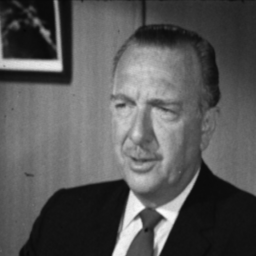
\includegraphics[width=0.4\textwidth]{gentelman_gray}
		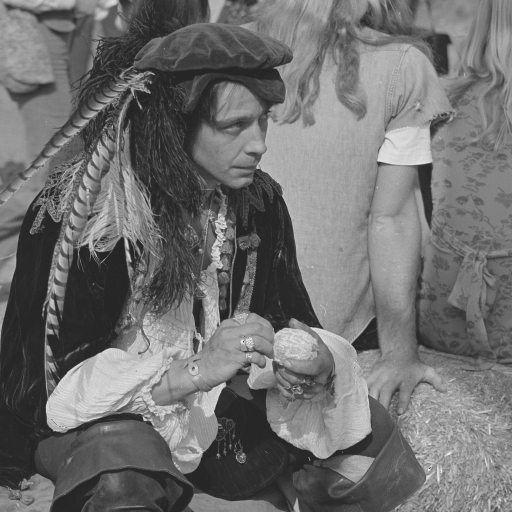
\includegraphics[width=0.4\textwidth]{pirate_gray}
	\end{center}
	\caption{Obrazy wejściowe (od lewej): obraz 1 (256x256), obraz 2 (512x512)}
\end{figure}

\begin{figure}[H]
	\begin{center}
		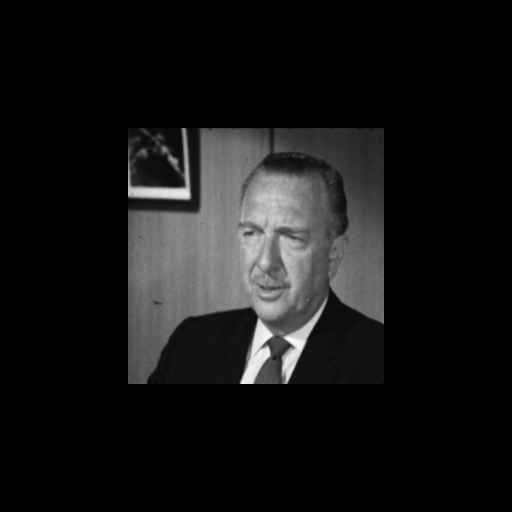
\includegraphics[width=0.4\textwidth]{gentelman_gray_unificationGeo_result}
		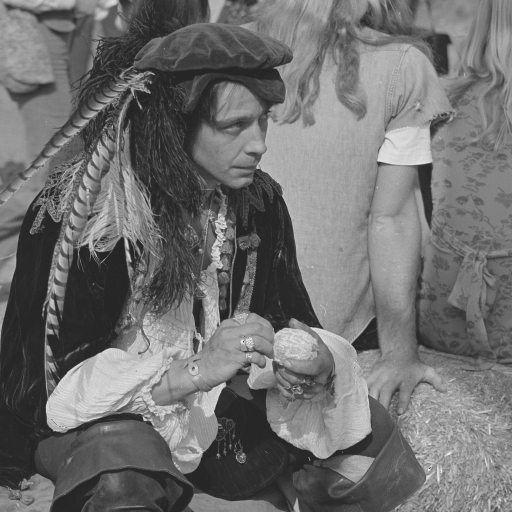
\includegraphics[width=0.4\textwidth]{pirate_gray_unificationGeo_result}
	\end{center}
	\caption{Obrazy wyjściowe (od lewej): obraz 1 (512x512), obraz 2 (512x512)}
\end{figure}

\subsection*{Kod źródłowy}
\hfill
\\\\
\noindent def geometricGray(self, show = False): \newline
\indent width1 = self.im1.shape[1] \newline
\indent width2 = self.im2.shape[1] \newline
\indent maxWidth = width1 $if$ width1 $>$ width2 $else$ width2 \newline

height1 = self.im1.shape[0] \newline
\indent height2 = self.im2.shape[0] \newline
\indent maxHeight = height1 $if$ height1 $>$ height2 $else$ height2 \newline

resultImage1 = np.empty((maxHeight, maxWidth), dtype = np.uint8)\newline
\indent resultImage2 = np.empty((maxHeight, maxWidth), dtype = np.uint8)\newline

startWidthCoord = int(round((maxWidth - width1) $//$ 2))\newline
\indent startHeightCoord = int(round((maxHeight - height1) $//$ 2))\newline

for i in range(0, maxHeight):\newline
\indent for j in range(0, maxWidth):\newline
\indent resultImage1[i, j] = 1\newline

\indent for i in range(0, height1):\newline
\indent for j in range(0, width1):\newline
\indent resultImage1[i + startHeightCoord, j + startWidthCoord] = self.im1[i, j]\newline

startWidthCoord = int(round((maxWidth - width2) $//$ 2))\newline
\indent startHeightCoord = int(round((maxHeight - height2) $//$ 2))\newline

for i in range(0, maxHeight):\newline
\indent for j in range(0, maxWidth):\newline
\indent resultImage2[i, j] = 1\newline

for i in range(0, height2):\newline
\indent for j in range(0, width2):\newline
\indent resultImage2[i + startHeightCoord, j + startWidthCoord] = self.im2[i, j]\newline

if show:\newline
\indent self.show(Image.fromarray(resultImage1, "L"), Image.fromarray(resultImage2, "L"))\newline
\indent self.save(resultImage1, self.im1Name, "unificationGeo")\newline
\indent self.save(resultImage2, self.im2Name, "unificationGeo")\newline

\newpage





\section*{2. Ujednolicenie obrazów szarych rozdzielczościowe}
\subsection*{Opis algorytmu}
\hfill
\\\\
\indent 
Operacja ujednolicania obrazów dzieli się na dwa etapy. Pierwszym jest ujednolicenie geometryczne, drugim zaś ujednolicenie rozdzielczościowe.

Operacja rozdzielczościowego ujednolicenia obrazów następuje po ujednoliceniu geometrycznym i polega na wypełnieniu obrazu pikslami, a brakujące piksle powinny być zinterpolowane.
\begin{enumerate}
	\item Wypełnij cały obraz pikslami o znanej wartości zachowując pewien odstęp między nimi.
	\item Każdemu pikslowi o nieznanej wartości przypisz zinterpolowaną wartość znanych piksli z jego bezpośredniego otoczenia.
\end{enumerate}

\begin{figure}[H]
	\begin{center}
		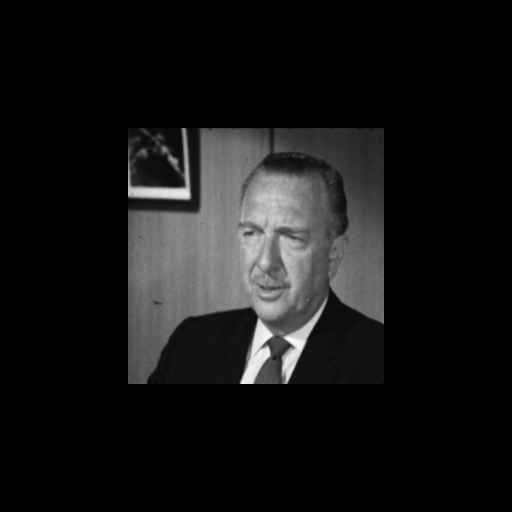
\includegraphics[width=0.35\textwidth]{gentelman_gray_unificationGeo_result}
		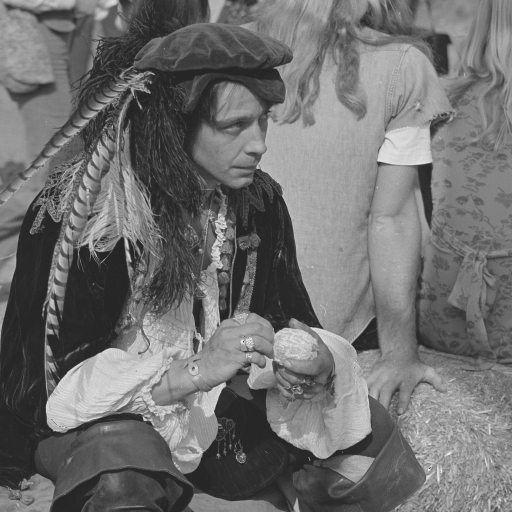
\includegraphics[width=0.35\textwidth]{pirate_gray_unificationGeo_result}
	\end{center}
	\caption{Obrazy wejściowe (od lewej): obraz 1 (512x512), obraz 2 (512x512)}
\end{figure}

\begin{figure}[H]
	\begin{center}
		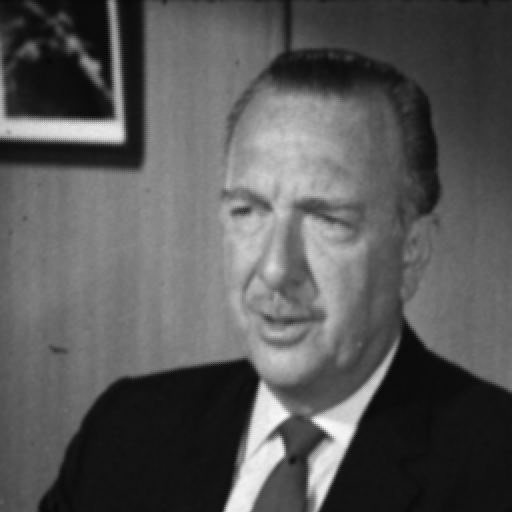
\includegraphics[width=0.35\textwidth]{gentelman_gray_unificationRas_result}
		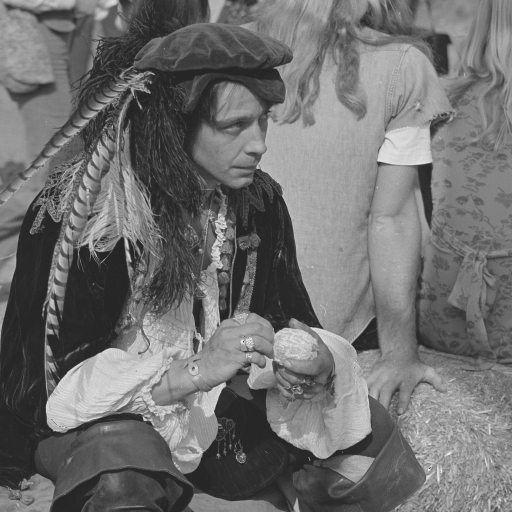
\includegraphics[width=0.35\textwidth]{pirate_gray_unificationRas_result}
	\end{center}
	\caption{Obrazy wyjściowe (od lewej): obraz 1 (512x512), obraz 2 (512x512)}
\end{figure}

\subsection*{Kod źródłowy}
\hfill
\\\\
\noindent def rasterGray(self, show = False):

width1 = self.im1.shape[1] \newline
\indent width2 = self.im2.shape[1] \newline

\indent height1 = self.im1.shape[0] \newline
\indent height2 = self.im2.shape[0] \newline

\indent scaleW = width1 $//$ width2 \newline
\indent scaleH = height1 $//$ height2 \newline

resultImage1 = np.zeros((height1, width1), dtype = np.uint8) \newline
\indent resultImage2 = np.zeros((height1, width1), dtype = np.uint8) \newline
\indent tmp = np.zeros((height1, width1), dtype = np.uint8) \newline

for i in range(height1): \newline
\indent for j in range(width1): \newline
\indent resultImage1[i, j] = self.im1[i, j] \newline

count = 0 \newline
\indent for i in range(height2): \newline
\indent for j in range(width2): \newline
\indent if count == 0: \newline
\indent resultImage2[int(scaleH*i), int(round(scaleW*j)) + 1] = self.im2[i, j] \newline
\indent count += 1 \newline
\indent if count == 1: \newline
\indent resultImage2[int(round(scaleH*i)) + 1, int(scaleW*j)] = self.im2[i, j] \newline
\indent count = 0 \newline

for i in range(height1): \newline
\indent for j in range(width1): \newline
\indent value = 0 \newline
\indent n = 0 \newline
\indent tmp[i, j] = resultImage2[i, j] \newline
\indent if resultImage2[i, j] $<$ 1: \newline
\indent for iOff in range(-1, 2): \newline
\indent for jOff in range(-1, 2): \newline
\indent iSafe = i if ((i + iOff) $>$ (height1 - 2)) $\mid$ ((i + iOff) < 0) else (i + iOff) \newline
\indent jSafe = j if ((j + jOff) $>$ (width1 - 2)) $\mid$ ((j + jOff) < 0) else (j + jOff) \newline
\indent if resultImage2[iSafe, jSafe] $>$ 0: \newline
\indent value += resultImage2[iSafe, jSafe] \newline
\indent n += 1 \newline
tmp[i, j] = value $//$ n \newline
resultImage2[i, j] = tmp[i, j] \newline

\noindent if show: \newline
self.show(Image.fromarray(resultImage1, "L"), Image.fromarray(resultImage2, "L")) \newline
self.save(resultImage1, self.im1Name, "unificationRas") \newline
self.save(resultImage2, self.im2Name, "unificationRas") \newline
\newpage







\section*{3. Ujednolicenie obrazów RGB geometryczne}
\subsection*{Opis algorytmu}
\hfill
\\\\
\indent 
Operacja ujednolicania obrazów dzieli się na dwa etapy. Pierwszym jest ujednolicenie geometryczne, drugim zaś ujednolicenie rozdzielczościowe.

Operacja geometrycznego ujednolicenia obrazów polega na doprowadzeniu obydwu obrazów do takiej samej liczby wierszy piksli w każdym obrazie i takiej samej liczby kolumn piksli w każdym obrazie.
\begin{enumerate}
	\item Wybierz największą wysokość i największą szerokość z dwuch obrazów.
	\item Jeśli dany obraz ma mniejszą szerokość albo wysokość, wypełnij różnicę pikslami o wartości 1 dla każdego z kanałów R, G i B (aby uniknąć dzielenia przez 0).
\end{enumerate}

\begin{figure}[H]
	\begin{center}
		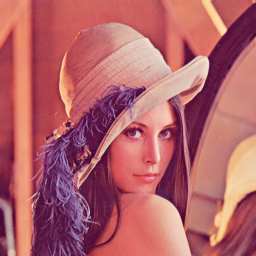
\includegraphics[width=0.4\textwidth]{lena_color}
		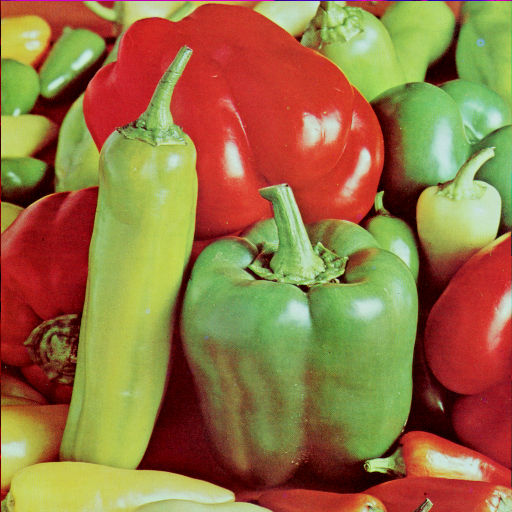
\includegraphics[width=0.4\textwidth]{peppers_color}
	\end{center}
	\caption{Obrazy wejściowe (od lewej): obraz 1 (256x256), obraz 2 (512x512)}
\end{figure}

\begin{figure}[H]
	\begin{center}
		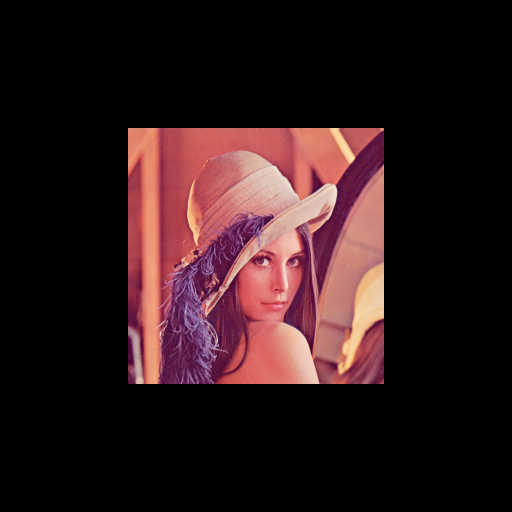
\includegraphics[width=0.4\textwidth]{lena_color_unificationGeo_result}
		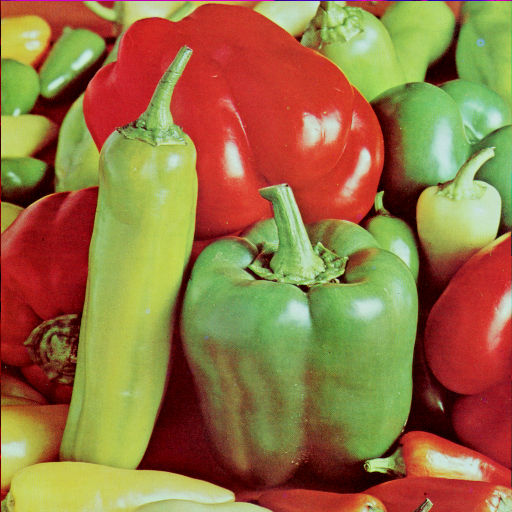
\includegraphics[width=0.4\textwidth]{peppers_color_unificationGeo_result}
	\end{center}
	\caption{Obrazy wyjściowe (od lewej): obraz 1 (512x512), obraz 2 (512x512)}
\end{figure}

\subsection*{Kod źródłowy}
\hfill
\\\\
\noindent def geometricColor(self, show = False): \newline
\indent width1 = self.im1.shape[1] \newline
\indent width2 = self.im2.shape[1] \newline
\indent maxWidth = width1 if width1 > width2 else width2 \newline

height1 = self.im1.shape[0] \newline
\indent height2 = self.im2.shape[0] \newline
\indent maxHeight = height1 if height1 > height2 else height2 \newline

resultImage1 = np.empty((maxHeight, maxWidth, 3), dtype = np.uint8) \newline
\indent resultImage2 = np.empty((maxHeight, maxWidth, 3), dtype = np.uint8) \newline

startWidthCoord = int(round((maxWidth - width1) $//$ 2)) \newline
\indent startHeightCoord = int(round((maxHeight - height1) $//$ 2)) \newline

for i in range(0, maxHeight): \newline
\indent for j in range(0, maxWidth): \newline
\indent resultImage1[i, j] = (1, 1, 1) \newline

for i in range(0, height1): \newline
\indent for j in range(0, width1): \newline
\indent resultImage1[i + startHeightCoord, j + startWidthCoord] = self.im1[i, j] \newline

startWidthCoord = int(round((maxWidth - width2) $//$ 2)) \newline
\indent startHeightCoord = int(round((maxHeight - height2) $//$ 2)) \newline

for i in range(0, maxHeight): \newline
\indent for j in range(0, maxWidth): \newline
\indent resultImage2[i, j] = (1, 1, 1) \newline

for i in range(0, height2): \newline
\indent for j in range(0, width2): \newline
\indent resultImage2[i + startHeightCoord, j + startWidthCoord] = self.im2[i, j] \newline

if show: \newline
\indent self.show(Image.fromarray(resultImage1, "RGB"), Image.fromarray(resultImage2, "RGB")) \newline
\indent self.save(resultImage1, self.im1Name, "unificationGeo") \newline
\indent self.save(resultImage2, self.im2Name, "unificationGeo") \newline
\newpage





\section*{4. Ujednolicenie obrazów RGB rozdzielczościowe}
\subsection*{Opis algorytmu}
\hfill
\\\\
\indent 
Operacja ujednolicania obrazów dzieli się na dwa etapy. Pierwszym jest ujednolicenie geometryczne, drugim zaś ujednolicenie rozdzielczościowe.

Operacja rozdzielczościowego ujednolicenia obrazów następuje po ujednoliceniu geometrycznym i polega na wypełnieniu obrazu pikslami, a brakujące piksle powinny być zinterpolowane.
\begin{enumerate}
	\item Wypełnij cały obraz pikslami o znanej wartości zachowując pewien odstęp między nimi.
	\item Każdemu pikslowi o nieznanej wartości przypisz zinterpolowaną wartość (dla każdego z kanałów R, G, B) znanych piksli z jego bezpośredniego otoczenia.
\end{enumerate}

\begin{figure}[H]
	\begin{center}
		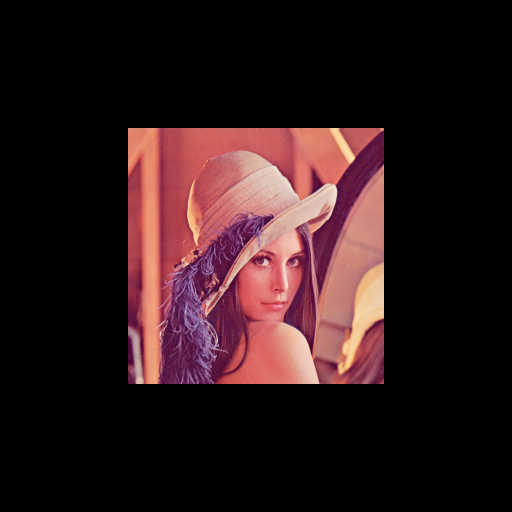
\includegraphics[width=0.4\textwidth]{lena_color_unificationGeo_result}
		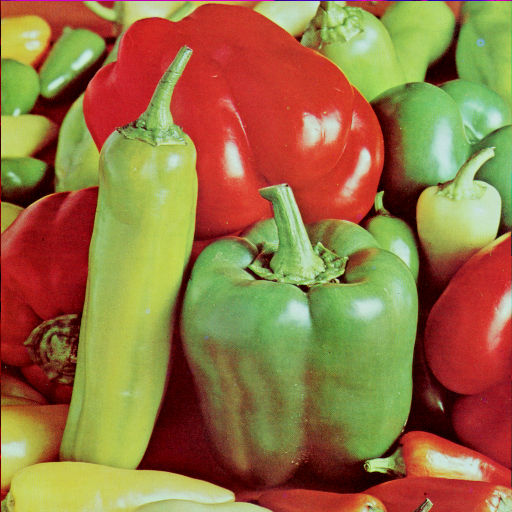
\includegraphics[width=0.4\textwidth]{peppers_color_unificationGeo_result}
	\end{center}
	\caption{Obrazy wejściowe (od lewej): obraz 1 (512x512), obraz 2 (512x512)}
\end{figure}

\begin{figure}[H]
	\begin{center}
		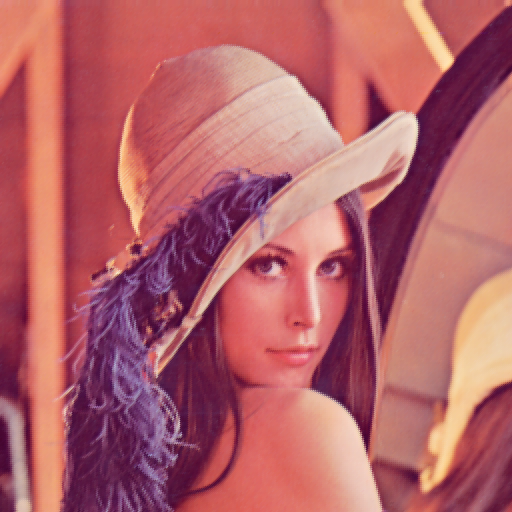
\includegraphics[width=0.4\textwidth]{lena_color_unificationRas_result}
		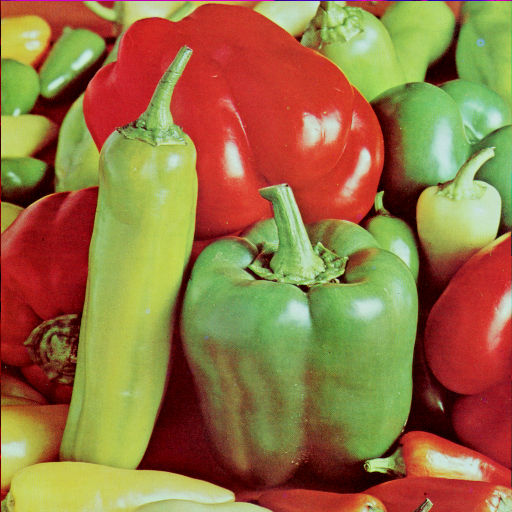
\includegraphics[width=0.4\textwidth]{peppers_color_unificationRas_result}
	\end{center}
	\caption{Obrazy wyjściowe (od lewej): obraz 1 (512x512), obraz 2 (512x512)}
\end{figure}

\subsection*{Kod źródłowy}
\hfill
\\\\
\noindent def rasterColor(self, show = False): \newline
\indent width1 = self.im1.shape[1] \newline
\indent width2 = self.im2.shape[1] \newline

height1 = self.im1.shape[0] \newline
\indent height2 = self.im2.shape[0] \newline

scaleW = width1 $//$ width2 \newline
\indent scaleH = height1 $//$ height2 \newline

resultImage1 = np.zeros((height1, width1, 3), dtype = np.uint8) \newline
\indent resultImage2 = np.zeros((height1, width1, 3), dtype = np.uint8) \newline
\indent tmp = np.zeros((height1, width1, 3), dtype = np.uint8) \newline

for i in range(height1): \newline
\indent for j in range(width1): \newline
\indent resultImage1[i, j] = self.im1[i, j] \newline

count = 0 \newline
\indent for i in range(height2): \newline
\indent for j in range(width2): \newline
\indent if count == 0: \newline
\indent resultImage2[int(scaleH*i), int(round(scaleW*j)) + 1] = self.im2[i, j] \newline
\indent count += 1 \newline
\indent if count == 1: \newline
\indent resultImage2[int(round(scaleH*i)) + 1, int(scaleW*j)] = self.im2[i, j] \newline
\indent count = 0 \newline

for i in range(height1): \newline
\indent for j in range(width1): \newline
\indent r, g, b = 0, 0, 0 \newline
\indent n = 0 \newline
\indent tmp[i, j] = resultImage2[i, j] \newline
\indent if (resultImage2[i, j][0] $<$ 1) $\&$ (resultImage2[i, j][1] $<$ 1) $\&$ (resultImage2[i, j][2] $<$ 1): \newline
\indent for iOff in range(-1, 2): \newline
\indent for jOff in range(-1, 2): \newline
\indent iSafe = i if ((i + iOff) > (height1 - 2)) $\mid$ ((i + iOff) < 0) else (i + iOff) \newline
\indent jSafe = j if ((j + jOff) > (width1 - 2)) $\mid$ ((j + jOff) < 0) else (j + jOff) \newline
\indent if (resultImage2[iSafe, jSafe][0] $>$ 0) $\mid$ (resultImage2[iSafe, jSafe][1] $>$ 0) $\mid$ (resultImage2[iSafe, jSafe][2] $>$ 0): \newline
\indent r += resultImage2[iSafe, jSafe][0] \newline
\indent \indent g += resultImage2[iSafe, jSafe][1] \newline
\indent \indent b += resultImage2[iSafe, jSafe][2] \newline
\indent \indent n += 1 \newline
\indent \indent tmp[i, j] = (r$//$n, g$//$n, b$//$n) \newline
\indent \indent resultImage2[i, j] = tmp[i, j] \newline

\indent \indent if show: \newline
\indent \indent self.show(Image.fromarray(resultImage1, "RGB"), Image.fromarray(resultImage2, "RGB")) \newline
\indent \indent self.save(resultImage1, self.im1Name, "unificationRas") \newline
\indent \indent self.save(resultImage2, self.im2Name, "unificationRas") \newline










\chapter{Operacje sumowania arytmetycznego obrazów szarych}
\section {Sumowanie (określonej) stałej z obrazem oraz dwóch obrazów}
\section {Mnożenie obrazu przez zadaną liczbę oraz przez inny obraz}
\section {Mieszanie obrazów z określonym współczynnikiem}
\section {Potęgowanie obrazu (z zadaną potęgą)}
\section {Dzielenie obrazu przez (zadaną) liczbę oraz przez inny obraz}
\section {Pierwiastkowanie obrazu}
\section {Logarytmowanie obrazu}

\chapter{Operacje sumowania arytmetycznego obrazów barwowych}
1. sumowanie (określonej) stałej z obrazem oraz dwóch obrazów
2. mnożenie obrazu przez zadaną liczbę oraz przez inny obraz
3. mieszanie obrazów z określonym współczynnikiem
4. potęgowanie obrazu (z zadaną potęgą)
5. dzielenie obrazu przez (zadaną) liczbę oraz przez inny obraz
6. pierwiastkowanie obrazu
7. logarytmowanie obrazu

\chapter{Operacje geometryczne na obrazie}
1. przemieszczenie obrazu o zadany wektor
2. jednorodne i niejednorodne skalowanie obrazu
3. obracanie obrazu o dowolny kąt
4. symetrie względem osi układu i zadanej prostej
5. wycinanie fragmentów obrazu
6. kopiowanie fragmentów obrazów

\chapter{Operacje na histogramie obrazu szarego}
\pagebreak
\section*{1. obliczanie histogramu}
\subsection*{Opis algorytmu}
\hfill
\\\\
\indent 
Histogram obrazu szarego jest wykresem częstości występowania wartości szarości piksli w obrazie tj.
przyporządkowuje liczbę piskli do danego poziomu szarości.\newline
\begin{enumerate}
	\item Zaalokuj tablicę 256 elementową (tyle, ile poziomów szarości w obrazie)
	\item Dla każdego piskla:
	\item Zinkrementuj element tablicy o indeksie równym pozionie szarości danego piskla
\end{enumerate}

\begin{figure}[H]
	\begin{center}
		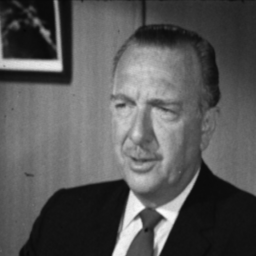
\includegraphics[width=0.4\textwidth]{gentelman_gray}
		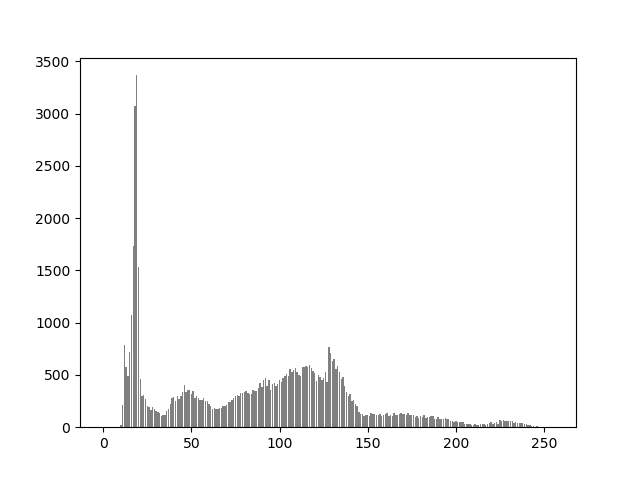
\includegraphics[width=0.4\textwidth]{gentelman_gray_histogram}
	\end{center}
	\caption{Obraz szary, histogram szarości tego obrazu}
\end{figure}

\begin{figure}[H]
	\begin{center}
		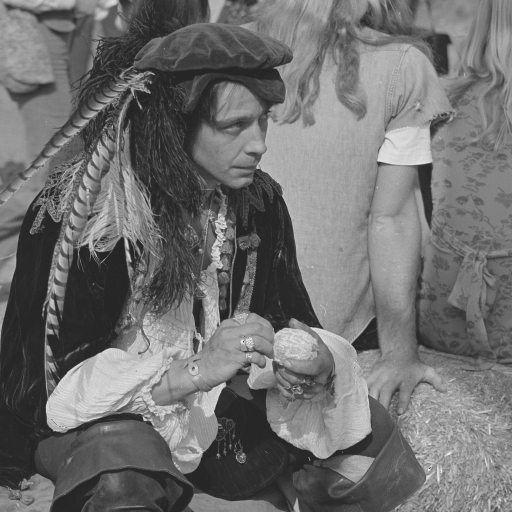
\includegraphics[width=0.4\textwidth]{pirate_gray}
		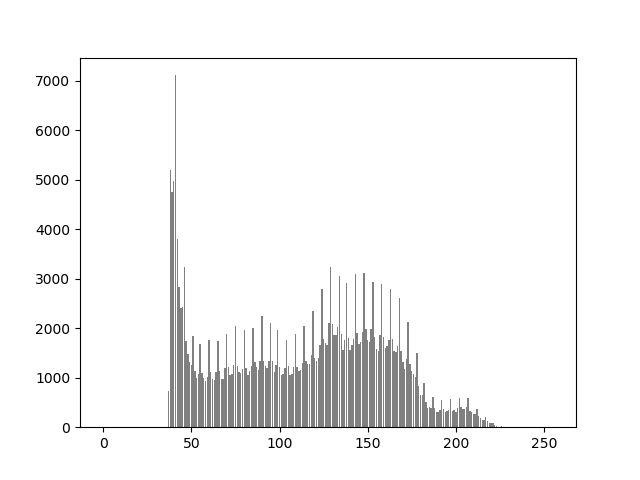
\includegraphics[width=0.4\textwidth]{pirate_gray_histogram}
	\end{center}
	\caption{Obraz szary, histogram szarości tego obrazu}
\end{figure}
\newpage

\subsection*{Kod źródłowy}
\hfill
\\\\
\noindent def calculate(self, plot = False, image = None): \newline
\indent if image is None: \newline
\indent image = self.im \newline

width = image.shape[1] \newline
\indent height = image.shape[0] \newline
\indent hist = [0] * 256 \newline

for i in range(height): \newline
\indent for j in range(width): \newline
\indent bin = image[i, j] \newline
\indent hist[bin] += 1 \newline

if plot: \newline
\indent bins = np.arange(256) \newline
\indent self.plotHistogram(bins, hist) \newline

return hist \newline
\newpage





\section*{2. przemieszczanie histogramu}
\subsection*{Opis algorytmu}
\hfill
\\\\
\indent Przemieszczenie histogramu polega na dodaniu lub odjęciu tej samej wartości od poziomu szarości każdego piksla w obrazie.
W rezultacie obraz jest odpowiednio równomiernie rozjaśniony bądź przyciemniony.
Nie można przekroczyć przyjętego zakresu poziomów szarości.
\begin{enumerate}
	\item Do każdej wartości piksla dodaj podaną stałą o którą chcesz przemieścić histogram.
	\item Jeśli wartość piksla po operacji dodawania wykracza poza zakres 255:
	\item Przypisz jej wartość 255.
	\item Jeśli wartość piksla po operacji dodawania jest mniejsza od 0:
	\item Przypisz jej wartość 0.
\end{enumerate}

\begin{figure}[H]
	\begin{center}
		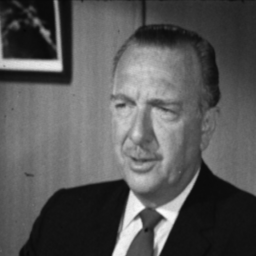
\includegraphics[width=0.4\textwidth]{gentelman_gray}
		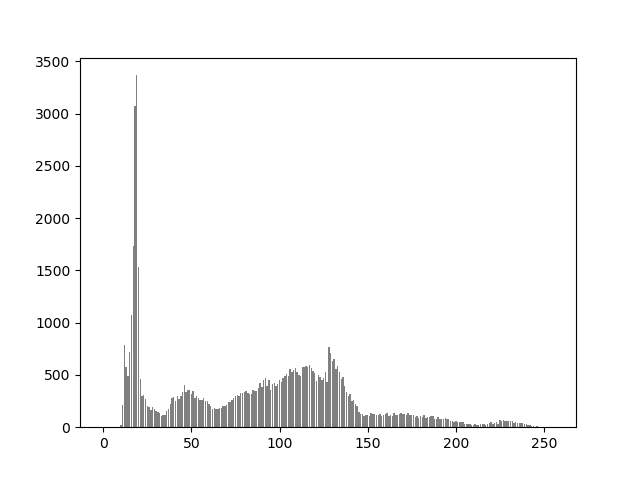
\includegraphics[width=0.4\textwidth]{gentelman_gray_histogram}
	\end{center}
	\caption{Obraz szary wejściowy, histogram szarości tego obrazu}
\end{figure}

\begin{figure}[H]
	\begin{center}
		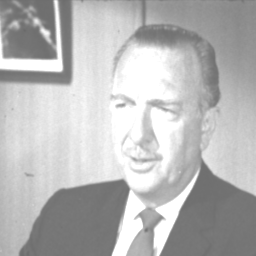
\includegraphics[width=0.4\textwidth]{gentelman_gray_moveHist_result}
		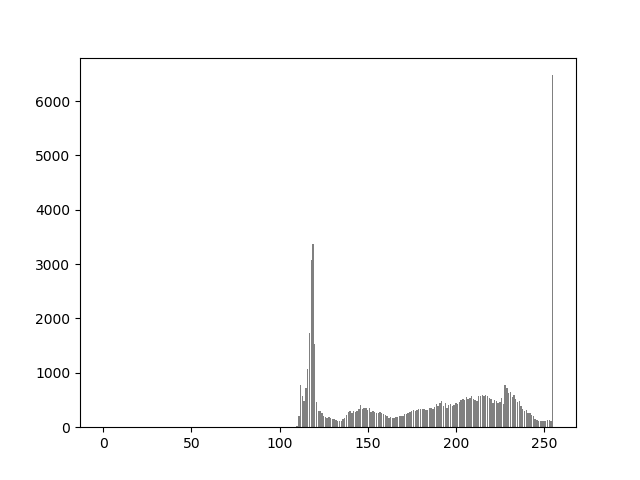
\includegraphics[width=0.4\textwidth]{gentelman_gray_moveHist_histogram}
	\end{center}
	\caption{Obraz szary przesunięty o 100, histogram szarości tego obrazu}
\end{figure}

\begin{figure}[t]
	\begin{center}
		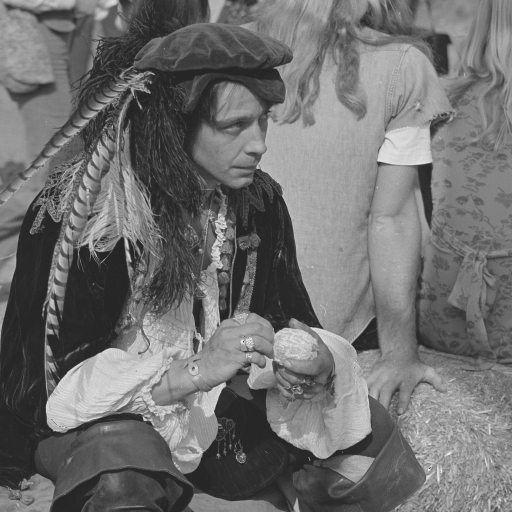
\includegraphics[width=0.4\textwidth]{pirate_gray}
		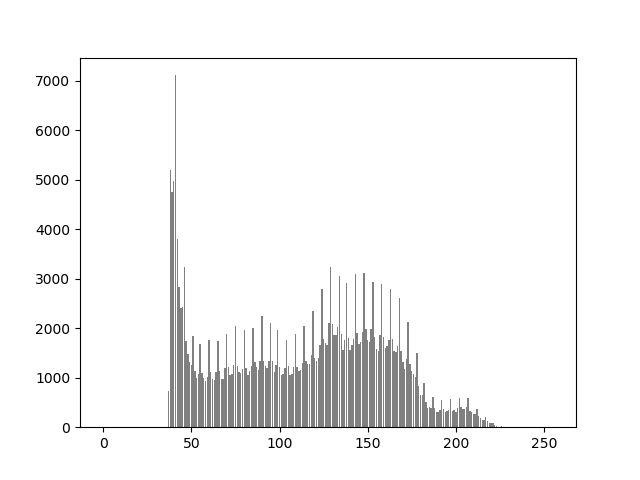
\includegraphics[width=0.4\textwidth]{pirate_gray_histogram}
	\end{center}
	\caption{Obraz szary wejściowy, histogram szarości tego obrazu}
\end{figure}

\begin{figure}[H]
	\begin{center}
		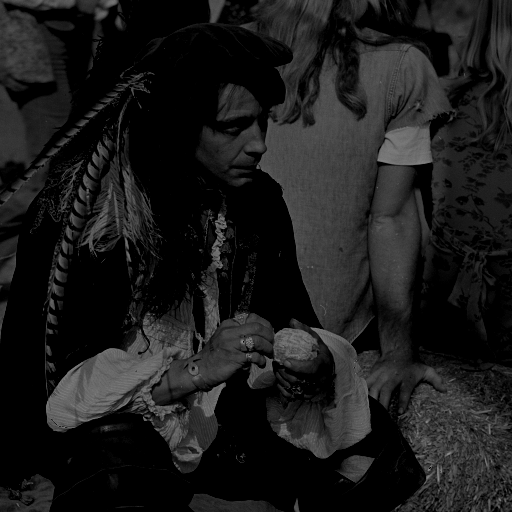
\includegraphics[width=0.4\textwidth]{pirate_gray_moveHist_result}
		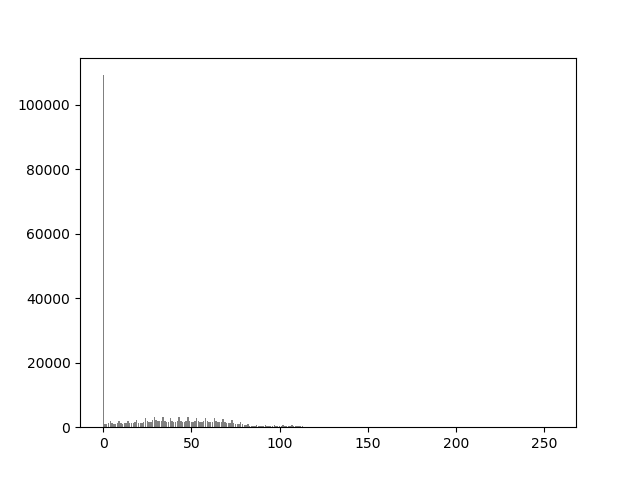
\includegraphics[width=0.4\textwidth]{pirate_gray_moveHist_histogram}
	\end{center}
	\caption{Obraz szary pryesunięty o -100, histogram szarości tego obrazu}
\end{figure}



\subsection*{Kod źródłowy}
\hfill
\\\\
\noindent def move(self, const = 0, show = False, plot = False): \newline
\indent width = self.im.shape[1] \newline
\indent height = self.im.shape[0] \newline

resultImage = np.empty((height, width), dtype=np.uint8) \newline

for i in range(height): \newline
\indent for j in range(width): \newline
\indent value = int(self.im[i, j]) + const \newline
\indent if value $<$ 0: \newline
\indent value = 0 \newline
elif value $>$ 255: \newline
value = 255 \newline
resultImage[i, j] = value \newline

\noindent if show: \newline
self.show(Image.fromarray(resultImage, "L")) \newline
self.calculate(plot, resultImage) \newline
self.save(resultImage, self.imName, "moveHist") \newline
\newpage





\section*{3. rozciąganie histogramu}
\subsection*{Opis algorytmu}
\hfill
\\\\
\indent Rozciągania histogramu dokonuje się na obrazie, którego poziomy szarości nie są rozpięte na cały możliwy zakres np.
[51, 233]. Operacja rozciągnięcia histogramu rozciągnie histogram tak, aby był rozpięty na cały możliwy zakres poziomów szarości np. [0, 255].
\begin{enumerate}
	\item Znajdź w obrazie największą($max$) i najmniejszą($min$) wartość piksla
	\item Dla każdego piksla:
	\item Oblicz nową wartość piskla stosując wzór:\\
	\centerline{$P_n = 255$ $//$ $(max - min) * (P_o - min)$.}
	W taki sposób, jeśli odcienie szarości obrazu wejściowego były w zakresie
	np. $[12, 239]$, po operacji rozciągania histogramu, odcienie szarości będą w zakresie\\
	$[0, 255]$
\end{enumerate}

\begin{figure}[H]
	\begin{center}
		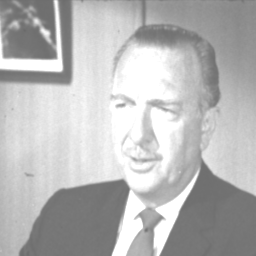
\includegraphics[width=0.35\textwidth]{gentelman_gray_moveHist_result}
		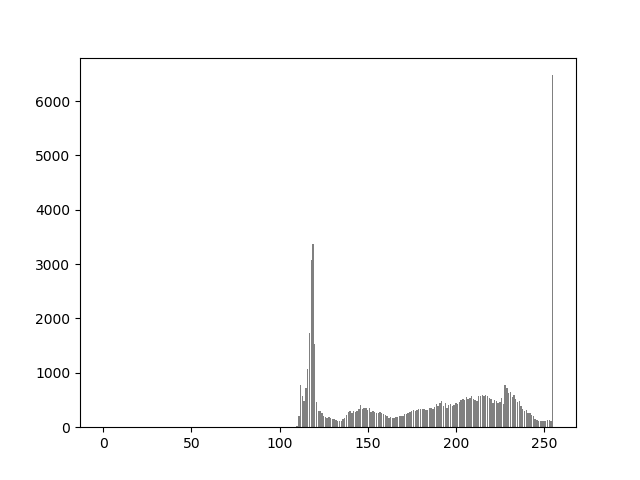
\includegraphics[width=0.35\textwidth]{gentelman_gray_moveHist_histogram}
	\end{center}
	\caption{Obraz wejściowy, histogram szarości tego obrazu}
\end{figure}

\begin{figure}[H]
	\begin{center}
		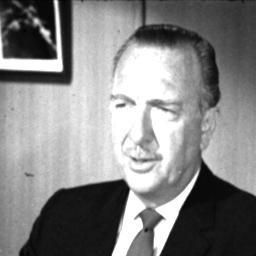
\includegraphics[width=0.35\textwidth]{gentelman_gray_stretchHist_result}
		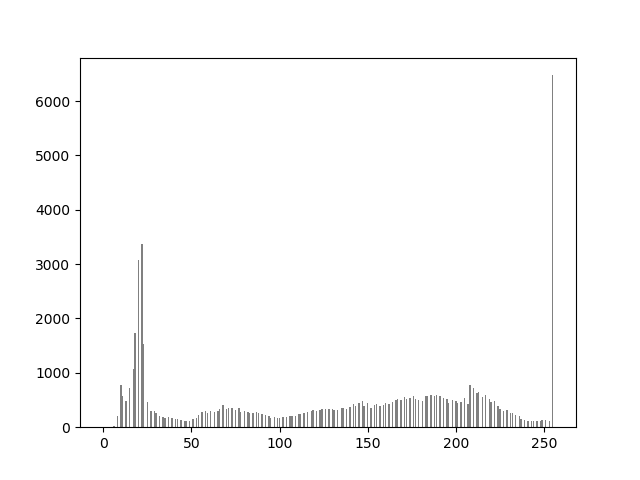
\includegraphics[width=0.35\textwidth]{gentelman_gray_stretchHist_histogram}
	\end{center}
	\caption{Obraz po rozciągnięciu, histogram szarości tego obrazu}
\end{figure}

\begin{figure}[H]
	\begin{center}
		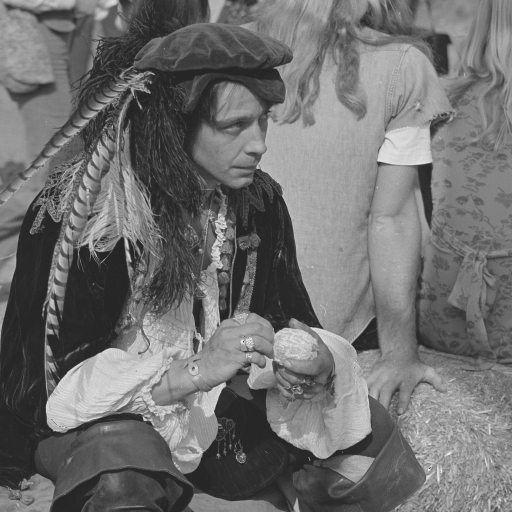
\includegraphics[width=0.35\textwidth]{pirate_gray}
		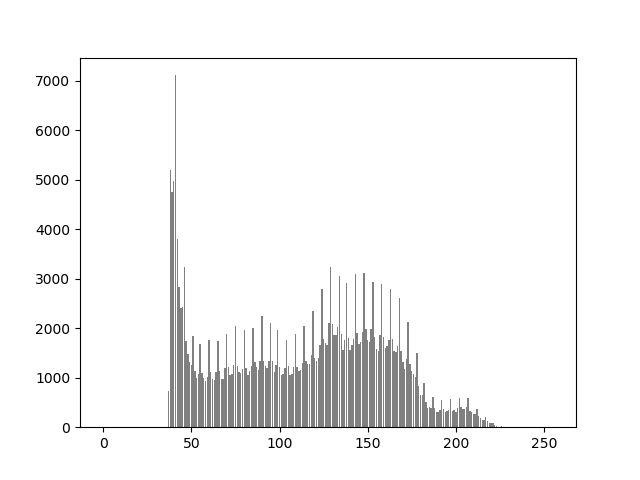
\includegraphics[width=0.35\textwidth]{pirate_gray_histogram}
	\end{center}
	\caption{Obraz wejściowy, histogram szarości tego obrazu}
\end{figure}

\begin{figure}[H]
	\begin{center}
		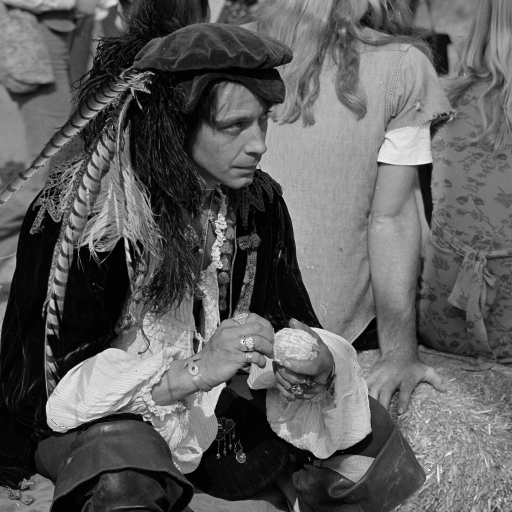
\includegraphics[width=0.35\textwidth]{pirate_gray_stretchHist_result}
		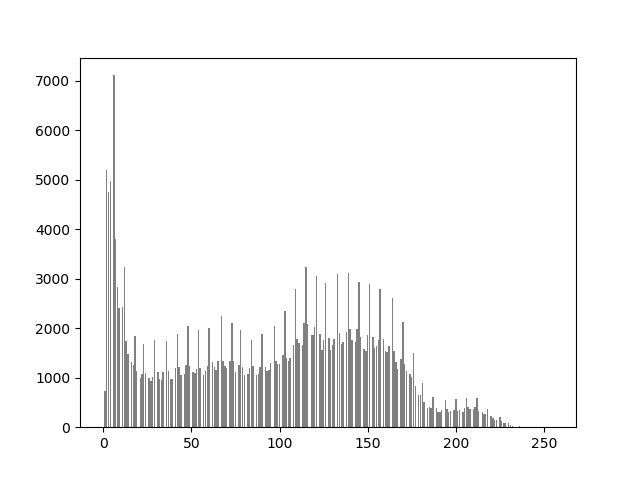
\includegraphics[width=0.35\textwidth]{pirate_gray_stretchHist_histogram}
	\end{center}
	\caption{Obraz po rozciągnięciu, histogram szarości tego obrazu}
\end{figure}

\subsection*{Kod źródłowy}
\hfill
\\\\
\noindent def stretch(self, show = False, plot = False):
\indent width = self.im.shape[1] \newline
\indent height = self.im.shape[0] \newline

resultImage = np.empty((height, width), dtype=np.uint8) \newline
\indent for i in range(height): \newline
\indent for j in range(width): \newline
\indent resultImage[i, j] = self.im[i, j] \newline

maxValue = 0 \newline
\indent minValue = 255 \newline
\indent while maxValue != 255: \newline

for i in range(height): \newline
\indent for j in range(width): \newline
\indent \indent \indent currValue = resultImage[i, j] \newline
\indent \indent \indent maxValue = max(maxValue, currValue) \newline
\indent \indent \indent minValue = min(minValue, currValue) \newline

\indent \indent \indent for i in range(height): \newline
\indent \indent \indent for j in range(width): \newline
\indent \indent \indent pix = resultImage[i, j] \newline
\indent \indent \indent resultImage[i, j] = ((255 $//$ (maxValue - minValue)) * (pix - minValue)) \newline

\indent \indent \indent if show: \newline
\indent \indent \indent self.show(Image.fromarray(resultImage, "L")) \newline
\indent \indent \indent self.calculate(plot, resultImage) \newline
\indent \indent \indent self.save(resultImage, self.imName, "stretchHist") \newline
\newpage





\section*{4. progowanie lokalne}
\subsection*{Opis algorytmu}
\hfill
\\\\
\indent Progowanie lokalne oblicza wartość progową dla każdego piksla z osobna. Jest to jedna z metod binaryzacji obrazu, która w wyniku dokładniej odwzorowuje kształt obiektu na obrazie.
\begin{enumerate}
	\item Zdefiniuj wielkość otoczenia piksla (musi być nieparzysta, po to, aby mógł istnieć piksel środkowy).
	\item Dla każdego piskla:
	\item Oblicz wartość progową jako średnią wartość piksli w otoczeniu danego piksla.
	\item Jeśli wartość piksla środkowego jest $< 0$:
	\item Przypisz mu wartość $0$.
	\item W przeciwnym przypadku przypisz mu wartość $255$.
\end{enumerate}

\begin{figure}[H]
	\begin{center}
		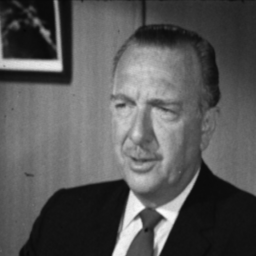
\includegraphics[width=0.37\textwidth]{gentelman_gray}
		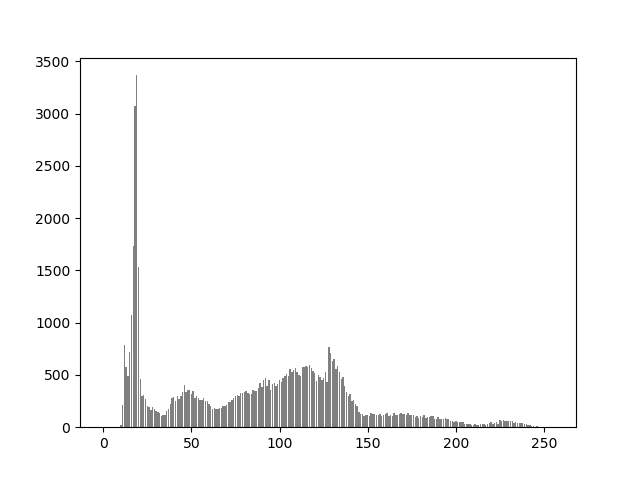
\includegraphics[width=0.37\textwidth]{gentelman_gray_histogram}
	\end{center}
	\caption{Obraz wejściowy, histogram szarości tego obrazu}
\end{figure}

\begin{figure}[H]
	\begin{center}
		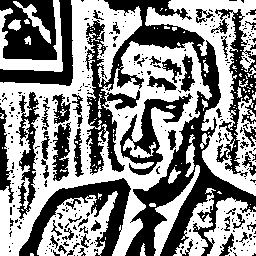
\includegraphics[width=0.37\textwidth]{gentelman_gray_locThreshold_result}
		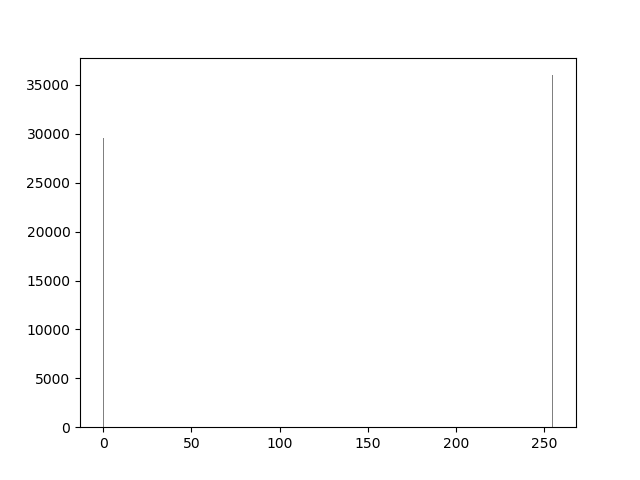
\includegraphics[width=0.37\textwidth]{gentelman_gray_locThreshold_histogram}
	\end{center}
	\caption{Obraz po progowaniu z parametrem 20, histogram szarości tego obrazu}
\end{figure}

\begin{figure}[H]
	\begin{center}
		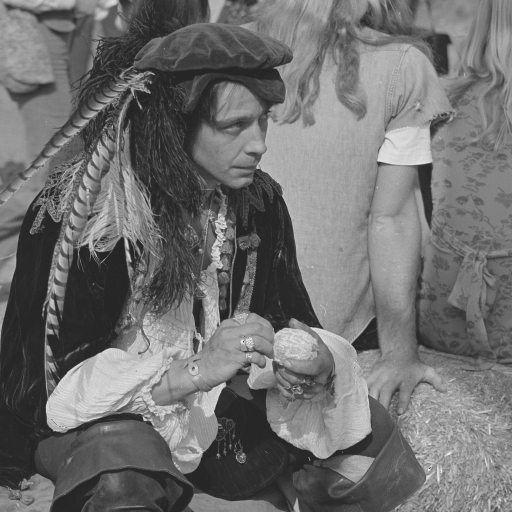
\includegraphics[width=0.4\textwidth]{pirate_gray}
		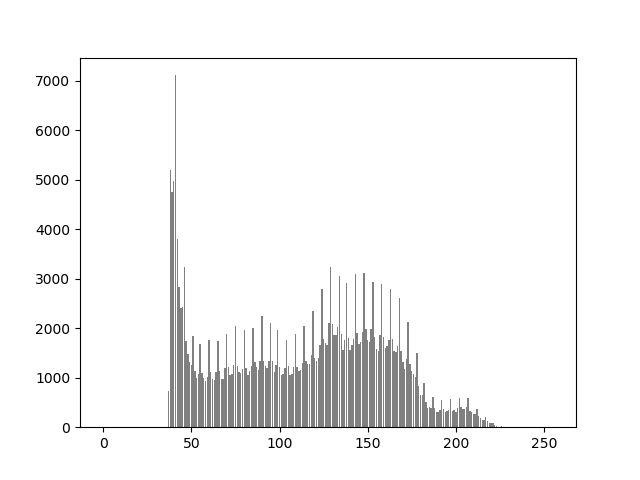
\includegraphics[width=0.4\textwidth]{pirate_gray_histogram}
	\end{center}
	\caption{Obraz wejściowy, histogram szarości tego obrazu}
\end{figure}

\begin{figure}[H]
	\begin{center}
		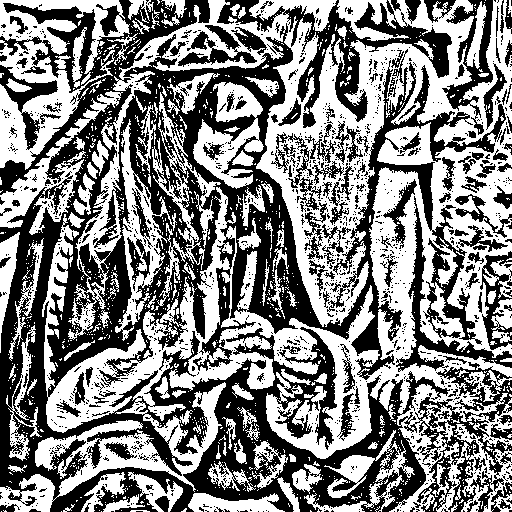
\includegraphics[width=0.4\textwidth]{pirate_gray_locThreshold_result}
		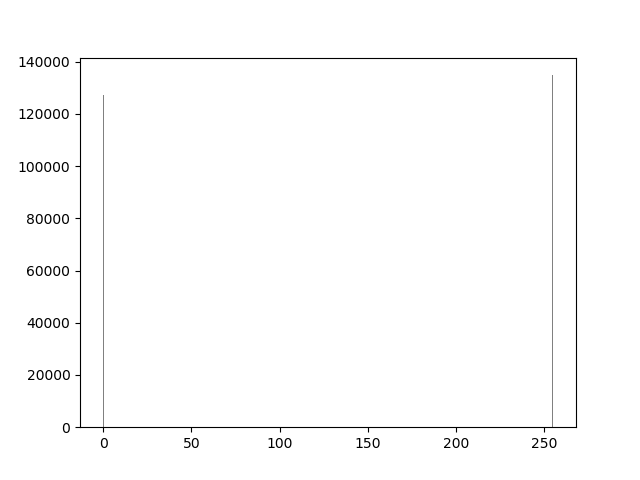
\includegraphics[width=0.4\textwidth]{pirate_gray_locThreshold_histogram}
	\end{center}
	\caption{Obraz po progowaniu z parametrem 20, histogram szarości tego obrazu}
\end{figure}

\subsection*{Kod źródłowy}
\hfill
\\\\
\noindent def localThreshold(self, dim = 3, show = False, plot = False): \newline
\indent width = self.im.shape[1] \newline
\indent height = self.im.shape[0] \newline
\indent l, r = -(int(round(dim $//$ 2))), int(round(dim $//$ 2) + 1)\newline

resultImage = np.empty((height, width), dtype=np.uint8) \newline

for i in range(height): \newline
\indent for j in range(width): \newline
\indent n = 0 \newline
\indent threshold = 0 \newline
currPix = self.im[i, j] \newline
for iOff in range(l, r): \newline
for jOff in range(l, r): \newline
iSafe = i $if$ ((i + iOff) $>$ (height + l)) $else$ (i + iOff) \newline
jSafe = j $if$ ((j + jOff) $>$ (width + l)) $else$ (j + jOff) \newline
threshold += self.im[iSafe, jSafe] \newline
n += 1 \newline
threshold = int(round(threshold / n)) \newline
resultImage[i, j] = 0 if (currPix $<$ threshold) else 255 \newline

\noindent if show: \newline
self.show(Image.fromarray(resultImage, "L")) \newline
self.calculate(plot, resultImage) \newline
self.save(resultImage, self.imName, "locThreshold") \newline
\newpage
\clearpage




\section*{5. progowanie globalne}
\subsection*{Opis algorytmu}
\hfill
\\\\
\indent Progowanie globalne jest jedną z metod binaryzacji obrazu. Wartość progowa jest ustalana globalnie biorąc pod uwagę wartość każdego piklsla w obrazie, po czym stosując wyliczony próg aby nadać nową wartość każdemu poikslowi obraz w wyniku jest binarny.
\begin{enumerate}
	\item Oblicz wartość progową $T$, jako średnią wartość z wszystkich piskli w obrazie
	\item Dla każdego piskla:
	\item Jeśli wartość danego piskla jest $< T$:
	\item przypisz mu wartość $0$.
	\item W przeciwnym przypadku przypisz mu wartość 255.
\end{enumerate}

\begin{figure}[H]
	\begin{center}
		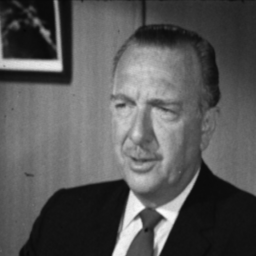
\includegraphics[width=0.4\textwidth]{gentelman_gray}
		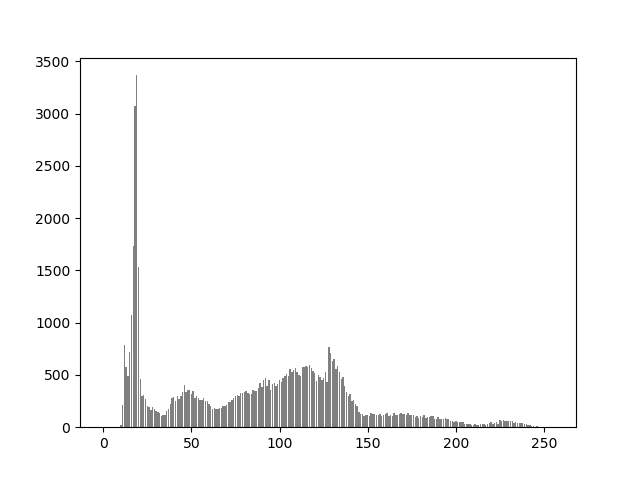
\includegraphics[width=0.4\textwidth]{gentelman_gray_histogram}
	\end{center}
	\caption{Obraz wejściowy, histogram szarości tego obrazu}
\end{figure}

\begin{figure}[H]
	\begin{center}
		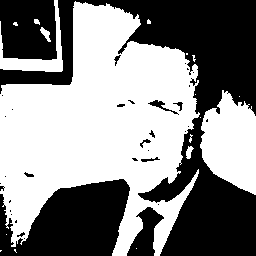
\includegraphics[width=0.4\textwidth]{gentelman_gray_globThreshold_result}
		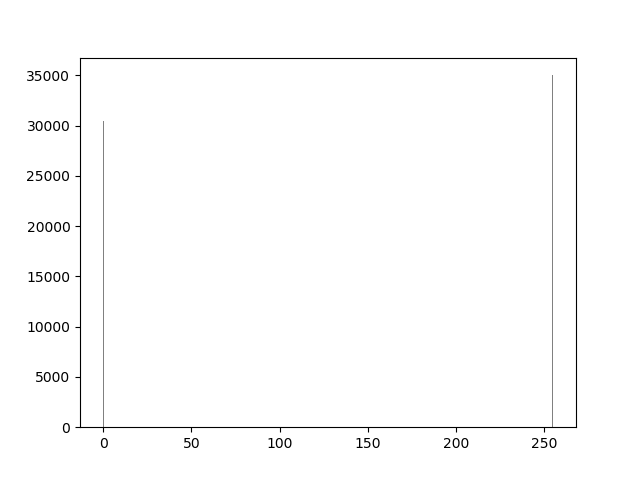
\includegraphics[width=0.4\textwidth]{gentelman_gray_globThreshold_histogram}
	\end{center}
	\caption{Obraz po progowaniu z parametrem 20, histogram szarości tego obrazu}
\end{figure}

\begin{figure}[H]
	\begin{center}
		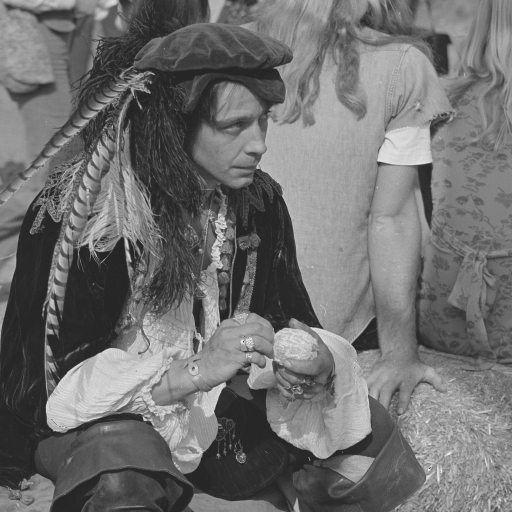
\includegraphics[width=0.4\textwidth]{pirate_gray}
		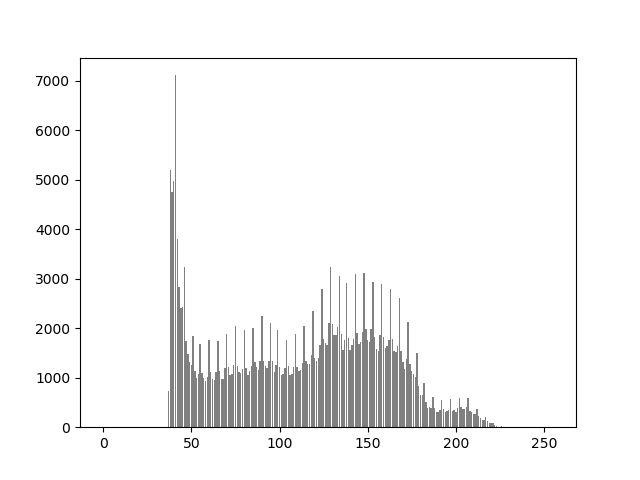
\includegraphics[width=0.4\textwidth]{pirate_gray_histogram}
	\end{center}
	\caption{Obraz wejściowy, histogram szarości tego obrazu}
\end{figure}

\begin{figure}[H]
	\begin{center}
		\includegraphics[width=0.4\textwidth]{pirate_gray_globThreshold_result}
		\includegraphics[width=0.4\textwidth]{pirate_gray_globThreshold_histogram}
	\end{center}
	\caption{Obraz po progowaniu z parametrem 20, histogram szarości tego obrazu}
\end{figure}

\subsection*{Kod źródłowy}
\hfill
\\\\
\noindent def globalThreshold(self, show = False, plot = False): \newline
\indent width = self.im.shape[1] \newline
\indent height = self.im.shape[0] \newline

resultImage = np.empty((height, width), dtype=np.uint8) \newline

threshold = 0 \newline
\indent n = 0 \newline
\indent for i in range(height): \newline
\indent for j in range(width): \newline
\indent threshold += self.im[i, j] \newline
\indent \indent \indent n += 1 \newline
\indent \indent \indent threshold = int(round(threshold / n)) \newline

\indent \indent \indent for i in range(height): \newline
\indent \indent \indent for j in range(width): \newline
\indent \indent \indent resultImage[i, j] = 0 if (self.im[i, j] < threshold) else 255 \newline

\indent \indent \indent if show: \newline
\indent \indent \indent self.show(Image.fromarray(resultImage, "L")) \newline
\indent \indent \indent self.calculate(plot, resultImage) \newline
\indent \indent \indent self.save(resultImage, self.imName, "globThreshold") \newline
\newpage






\chapter{Operacje na histogramie obrazu barwowego}
\pagebreak
\section*{1. obliczanie histogramu}
\subsection*{Opis algorytmu}
\hfill
\\\\
\indent Histogram obrazu barwnego jest wykresem częstości występowania wartości barwy piksli w obrazie tj.
przyporządkowuje liczbę piskli do danego poziomu barwy.\newline
\begin{enumerate}
	\item Zaalokuj 3 tablice 256 elementowe (tyle, ile poziomów barw w obrazie)
	\item Dla każdego piskla:
	\item Dla każdej barwy:
	\item Zinkrementuj element tablicy danej barwy o indeksie równym poziomie tej barwy danego piskla
\end{enumerate}

\begin{figure}[H]
	\begin{center}
		\includegraphics[width=0.4\textwidth]{lena_color}
		\includegraphics[width=0.4\textwidth]{lena_color_histogram}
	\end{center}
	\caption{Obraz barwny, histogram barw tego obrazu}
\end{figure}

\begin{figure}[H]
	\begin{center}
		\includegraphics[width=0.4\textwidth]{peppers_color}
		\includegraphics[width=0.4\textwidth]{peppers_color_histogram}
	\end{center}
	\caption{Obraz barwny, histogram barw tego obrazu}
\end{figure}
\pagebreak

\subsection*{Kod źródłowy}
\hfill
\\\\
\noindent def calculate(self, plot = False, image = None): \newline
\indent if image is None: \newline
\indent image = self.im \newline

width = image.shape[1] \newline
\indent height = image.shape[0] \newline
\indent hist = [0] * 3 \newline
\indent hist[0] = [0] * 256 \newline
\indent hist[1] = [0] * 256 \newline
\indent hist[2] = [0] * 256 \newline

for i in range(height): \newline
\indent for j in range(width): \newline
\indent bin = image[i, j] \newline
\indent for k in range(3): \newline
\indent hist[k][bin[k]] += 1 \newline

if plot: \newline
\indent bins = np.arange(256) \newline
\indent self.plotHistogram(bins, hist) \newline

return hist \newline
\pagebreak


\section*{2. Przemieszczanie histogramu}
\subsection*{Opis algorytmu}
\hfill
\\\\
\indent Przemieszczenie histogramu polega na dodaniu lub odjęciu tej samej wartości od poziomu każdej z barw każdego piksla w obrazie.
W rezultacie obraz jest odpowiednio równomiernie rozjaśniony bądź przyciemniony.
Nie można przekroczyć przyjętego zakresu poziomu barwy.
\begin{enumerate}
	\item Do każdej wartości barwy piksla dodaj podaną stałą, o którą chcesz przemieścić histogram.
	\item Jeśli wartość barwy piksla po operacji dodawania wykracza poza zakres 255:
	\item Przypisz jej wartość 255.
	\item Jeśli wartość piksla po operacji dodawania jest mniejsza od 0:
	\item Przypisz jej wartość 0.
\end{enumerate}

\begin{figure}[H]
	\begin{center}
		\includegraphics[width=0.35\textwidth]{lena_color}
		\includegraphics[width=0.35\textwidth]{lena_color_histogram}
	\end{center}
	\caption{Obraz wejściowy, histogram barw tego obrazu}
\end{figure}

\begin{figure}[H]
	\begin{center}
		\includegraphics[width=0.35\textwidth]{lena_color_moveHist_result}
		\includegraphics[width=0.35\textwidth]{lena_color_moveHist_histogram}
	\end{center}
	\caption{Obraz wyjściowy przesunięty o 50, histogram barw tego obrazu}
\end{figure}

\begin{figure}[H]
	\begin{center}
		\includegraphics[width=0.35\textwidth]{peppers_color}
		\includegraphics[width=0.35\textwidth]{peppers_color_histogram}
	\end{center}
	\caption{Obraz wejściowy, histogram barw tego obrazu}
\end{figure}

\begin{figure}[H]
	\begin{center}
		\includegraphics[width=0.35\textwidth]{peppers_color_moveHist_result}
		\includegraphics[width=0.35\textwidth]{peppers_color_moveHist_histogram}
	\end{center}
	\caption{Obraz wyjściowy przesunięty o -50, histogram barw tego obrazu}
\end{figure}


\subsection*{Kod źródłowy}
\hfill
\\\\
\noindent def move(self, const = 0, show = False, plot = False): \newline
\indent width = self.im.shape[1] \newline
\indent height = self.im.shape[0] \newline

resultImage = np.empty((height, width, 3), dtype=np.uint8) \newline

\indent for i in range(height): \newline
\indent for j in range(width): \newline
\indent value = self.im[i, j] \newline
\indent for k in range(len(value)): \newline
\indent v = value[k] \newline
\indent v += const \newline
\indent if v $<$ 0: \newline
\indent v = 0 \newline
\indent \indent \indent elif v $>$ 255: \newline
\indent \indent \indent v = 255 \newline
\indent \indent \indent value[k] = v \newline
\indent \indent \indent resultImage[i, j] = value \newline

\indent \indent \indent if show: \newline
\indent \indent \indent self.show(Image.fromarray(resultImage, "RGB")) \newline
\indent \indent \indent self.calculate(plot, resultImage) \newline
\indent \indent \indent self.save(resultImage, self.imName, "moveHist") \newline
\newpage

\section*{3. Rozciąganie histogramu}
\subsection*{Opis algorytmu}
\hfill
\\\\
\indent  Rozciągania histogramu dokonuje się na obrazie, którego poziomy barw nie są rozpięte na cały możliwy zakres np.
[51, 233]. Operacja rozciągnięcia histogramu rozciągnie histogram tak, aby był rozpięty na cały możliwy zakres poziomów barw np. [0, 255].
\begin{enumerate}
	\item Znajdź w obrazie największą($max_c$) i najmniejszą($min_c$) wartość piksla dla każdej z barw($c$)
	\item Dla każdego piksla($P_o$):
	\item Dla każdej z barw($c$):
	\item Oblicz nową wartość piskla($P_n$) stosując wzór:\\
	\centerline{$P_n = 255$ $//$ $(max_c - min_c) * (P_o - min_c)$.}
	W taki sposób, jeśli barwy obrazu wejściowego były w zakresie
	np. $[12, 239]$, po operacji rozciągania histogramu, będą w zakresie $[0, 255]$.
\end{enumerate}

\begin{figure}[H]
	\begin{center}
		\includegraphics[width=0.35\textwidth]{lena_color}
		\includegraphics[width=0.35\textwidth]{lena_color_histogram}
	\end{center}
	\caption{Obraz wejściowy, histogram barw tego obrazu}
\end{figure}

\begin{figure}[H]
	\begin{center}
		\includegraphics[width=0.35\textwidth]{lena_color_stretchHist_result}
		\includegraphics[width=0.35\textwidth]{lena_color_stretchHist_histogram}
	\end{center}
	\caption{Obraz po rozciągnięciu, histogram barw tego obrazu}
\end{figure}

\begin{figure}[H]
	\begin{center}
		\includegraphics[width=0.35\textwidth]{peppers_color}
		\includegraphics[width=0.35\textwidth]{peppers_color_histogram}
	\end{center}
	\caption{Obraz wejściowy, histogram barw tego obrazu}
\end{figure}

\begin{figure}[H]
	\begin{center}
		\includegraphics[width=0.35\textwidth]{peppers_color_stretchHist_result}
		\includegraphics[width=0.35\textwidth]{peppers_color_stretchHist_histogram}
	\end{center}
	\caption{Obraz po rozciągnięciu, histogram barw tego obrazu}
\end{figure}

\subsection*{Kod źródłowy}
\hfill
\\\\
\noindent def stretch(self, show = False, plot = False): \newline
\indent width = self.im.shape[1] \newline
\indent height = self.im.shape[0] \newline

resultImage = np.empty((height, width, 3), dtype=np.uint8) \newline
\indent for i in range(height): \newline
\indent for j in range(width): \newline
\indent resultImage[i, j] = self.im[i, j] \newline


maxValue = [0] * 3 \newline
\indent minValue = [255] * 3 \newline
\indent while (maxValue[0] != 255) $\&$ (maxValue[1] != 255) $\&$ (maxValue[2] != 255): \newline

\noindent for i in range(height): \newline
for j in range(width): \newline
currValue = resultImage[i, j] \newline
for k in range(3): \newline
maxValue[k] = max(maxValue[k], currValue[k]) \newline
minValue[k] = min(minValue[k], currValue[k]) \newline

\noindent for i in range(height): \newline
for j in range(width): \newline
pix = resultImage[i, j] \newline
for k in range(3): \newline
pix[k] = ((255 $//$ (maxValue[k] - minValue[k])) * (pix[k] - minValue[k])) \newline
resultImage[i, j] = pix \newline

\noindent if show: \newline
self.show(Image.fromarray(resultImage, "RGB")) \newline
self.calculate(plot, resultImage) \newline
self.save(resultImage, self.imName, "stretchHist") \newline
\newpage

\section*{4. Progowanie 1-progowe}
\subsection*{Opis algorytmu}
\hfill
\\\\
\indent 
\begin{enumerate}
	\item 
\end{enumerate}

\newpage

\section*{5. Progowanie wielo-progowe}
\subsection*{Opis algorytmu}
\hfill
\\\\
\indent 
\begin{enumerate}
	\item 
\end{enumerate}
\newpage

\section*{6. progowanie lokalne}
\subsection*{Opis algorytmu}
\hfill
\\\\
\indent Progowanie lokalne oblicza wartość progową dla każdego piksla z osobna. W wyniku takiego progowania obraz dokładniej odwzorowuje kształt obiektu.
\begin{enumerate}
	\item Zdefiniuj wielkość otoczenia piksla (musi być nieparzysta, po to, aby mógł istnieć piksel środkowy).
	\item Przenieś obraz do przestrzeni HSI.
	\item Dla każdego piskla($P$):
	\item Oblicz wartość progową składowej $I$ jako średnią wartość piksli w otoczeniu danego piksla($P$).
	\item Jeśli wartość skłądowej $I$ piksla $P$ jest $< 0$:
	\item Przypisz mu wartość $0$.
	\item W przeciwnym przypadku przypisz mu wartość $1$.
	\item Przenieś obraz spowrotem do przestrzeni RGB.
\end{enumerate}

\begin{figure}[H]
	\begin{center}
		\includegraphics[width=0.35\textwidth]{lena_color}
		\includegraphics[width=0.35\textwidth]{lena_color_histogram}
	\end{center}
	\caption{Obraz wejściowy, histogram szarości tego obrazu}
\end{figure}

\begin{figure}[H]
	\begin{center}
		\includegraphics[width=0.35\textwidth]{lena_color_locThreshold_result}
		\includegraphics[width=0.35\textwidth]{lena_color_locThreshold_histogram}
	\end{center}
	\caption{Obraz po progowaniu z otoczeniem piksla 21x21, histogram szarości tego obrazu}
\end{figure}

\begin{figure}[H]
	\begin{center}
		\includegraphics[width=0.35\textwidth]{peppers_color}
		\includegraphics[width=0.35\textwidth]{peppers_color_histogram}
	\end{center}
	\caption{Obraz wejściowy, histogram szarości tego obrazu}
\end{figure}

\begin{figure}[H]
	\begin{center}
		\includegraphics[width=0.35\textwidth]{peppers_color_locThreshold_result}
		\includegraphics[width=0.35\textwidth]{peppers_color_locThreshold_histogram}
	\end{center}
	\caption{Obraz po progowaniu z otoczeniem piksla 21x21, histogram szarości tego obrazu}
\end{figure}

\subsection*{Kod źródłowy}
\hfill
\\\\
\noindent def localThreshold(self, dim = 3, show = False, plot = False): \newline
\indent width = self.im.shape[1] \newline
\indent height = self.im.shape[0] \newline
\indent low, up = -(int(round(dim $//$ 2))), int(round(dim $//$ 2) + 1) \newline

resultImage = np.empty((height, width, 3), dtype=np.uint8) \newline
\indent tmp = np.empty((height, width, 3)) \newline
\indent tmp2 = np.empty((height, width, 3)) \newline


for i in range(height): \newline
\indent for j in range(width): \newline
\indent r, g, b = self.im[i, j] \newline
\indent tmp[i, j] = self.RGBtoHSI((r, g, b)) \newline

\indent for i in range(height): \newline
\indent for j in range(width): \newline
\indent H = 0 \newline
\indent n = 0 \newline
\indent currPix = tmp[i, j] \newline
\indent for iOff in range(low, up): \newline
\indent for jOff in range(low, up): \newline
\indent iSafe = i $if$ ((i + iOff) $>$ (height + low)) $\mid$ ((i + iOff) $<$ 0) $else$ (i + iOff) \newline
\indent jSafe = j $if$ ((j + jOff) $>$ (width + low)) $\mid$ ((j + jOff) $<$ 0) $else$ (j + jOff) \newline
\indent H += tmp[iSafe, jSafe][2] \newline
\indent n += 1 \newline
\indent H = H $//$ n \newline
\indent tmp2[i, j] = currPix \newline
\indent tmp2[i, j][2] = 0 $if$ currPix[2] $<$ H $else$ 1 \newline

\indent for i in range(height): \newline
\indent for j in range(width): \newline
\indent h, s, I = tmp2[i, j] \newline
\indent resultImage[i, j] = self.HSItoRGB((h, s, I)) \newline

\indent if show: \newline
\indent self.show(Image.fromarray(resultImage, "RGB")) \newline
\indent self.calculate(plot, resultImage) \newline
\indent self.save(resultImage, self.imName, "locThreshold") \newline
\newpage

\section*{7. Progowanie globalne}
\subsection*{Opis algorytmu}
\hfill
\\\\
\indent W progowaniu globalnym wartość progowa jest ustalana globalnie, biorąc pod uwagę wartość składowej intensywnościowej (z przestrzeni HSI) każdego piklsla w obrazie. Następnie, tak wyliczona wartość progowa, jest stosowana do nadania każdemu pikslowi nową wartość.
\begin{enumerate}
	\item Przenieś obraz do przestrzeni HSI.
	\item Oblicz wartość progową $T$, jako średnią wartość składowej intensywnościowej ($I$) z wszystkich piskli w obrazie.
	\item Dla każdego piskla:
	\item Jeśli wartość $I$ danego piskla jest $< T$:
	\item przypisz mu wartość $0$.
	\item W przeciwnym przypadku przypisz mu wartość 1.
	\item Przenieś obraz spowrotem do przestrzeni RGB.
\end{enumerate}

\begin{figure}[H]
	\begin{center}
		\includegraphics[width=0.35\textwidth]{lena_color}
		\includegraphics[width=0.35\textwidth]{lena_color_histogram}
	\end{center}
	\caption{Obraz wejściowy, histogram barw tego obrazu}
\end{figure}

\begin{figure}[H]
	\begin{center}
		\includegraphics[width=0.35\textwidth]{lena_color_globThreshold_result}
		\includegraphics[width=0.35\textwidth]{lena_color_globThreshold_histogram}
	\end{center}
	\caption{Obraz po progowaniu globalnym, histogram barw tego obrazu}
\end{figure}

\begin{figure}[H]
	\begin{center}
		\includegraphics[width=0.35\textwidth]{peppers_color}
		\includegraphics[width=0.35\textwidth]{peppers_color_histogram}
	\end{center}
	\caption{Obraz wejściowy, histogram barw tego obrazu}
\end{figure}

\begin{figure}[H]
	\begin{center}
		\includegraphics[width=0.35\textwidth]{peppers_color_globThreshold_result}
		\includegraphics[width=0.35\textwidth]{peppers_color_globThreshold_histogram}
	\end{center}
	\caption{Obraz po progowaniu globalnym, histogram barw tego obrazu}
\end{figure}

\subsection*{Kod źródłowy}
\hfill
\\\\
\noindent def globalThreshold(self, show = False, plot = False): \newline
\indent width = self.im.shape[1] \newline
\indent height = self.im.shape[0] \newline

resultImage = np.empty((height, width, 3), dtype=np.uint8) \newline
\indent tmp = np.empty((height, width, 3)) \newline
\indent tmp2 = np.empty((height, width, 3)) \newline


\indent for i in range(height): \newline
\indent for j in range(width): \newline
\indent r, g, b = self.im[i, j] \newline
\indent tmp[i, j] = self.RGBtoHSI((r, g, b)) \newline

\noindent H = 0 \newline
n = 0 \newline
for i in range(height): \newline
for j in range(width): \newline
H += tmp[i, j][2] \newline
n += 1 \newline
H = H $//$ n \newline

\noindent for i in range(height): \newline
for j in range(width): \newline
tmp2[i, j] = tmp[i, j] \newline
tmp2[i, j][2] = 0 if tmp[i, j][2] $<$ H else 1 \newline

\noindent for i in range(height): \newline
for j in range(width): \newline
h, s, I = tmp2[i, j] \newline
resultImage[i, j] = self.HSItoRGB((h, s, I)) \newline

\noindent if show: \newline
self.show(Image.fromarray(resultImage, "RGB")) \newline
self.calculate(plot, resultImage) \newline
self.save(resultImage, self.imName, "globThreshold") \newline
\newpage


\chapter{Operacje morfologiczne na obrazach binarnych}
1. okrawanie(erozja)
2. nakładanie (dylatacja)
3. otwarcie
4. zamknięcie

\chapter {Operacje morfologiczne na obrazach szarych}
1. okrawanie(erozja)
2. nakładanie (dylatacja)
3. otwarcie
4. zamknięcie

\chapter {Filtrowanie liniowe i nieliniowe}
\newpage


\section*{1.1 Filtr dolnoprzepustowy uśredniający}
\subsection*{Opis algorytmu}
\hfill
\\\\
\indent Filtr uśredniający jest podstawowym filtrem dolnoprzepustowym, jego wynikiem jest uśrednienie każdego piksla razem ze swoimi sąsiadami. Maska:
\begin{center}
	$\frac{1}{9}$ 
	\begin{tabular}{|c|c|c|}
		\hline
		1 & 1 & 1\\
		\hline
		1 & 1 & 1\\
		\hline
		1 & 1 & 1\\
		\hline
	\end{tabular}
\end{center}

\begin{enumerate}
	\item Dla każdego piksla($P$):
	\item Dla każdej barwy:
	\item Zsumuj wartości barwy piksli, otaczających piksel $P$ pomnożonych przez odpowiednią wagę maski.
	\item Sumę barwy podziel przez sumę wag maski.
	\item Przypisz nową wartość barwy pikslowi $P$.
\end{enumerate}

\begin{figure}[H]
	\begin{center}
		\includegraphics[width=0.35\textwidth]{gentelman_gray}
		\includegraphics[width=0.35\textwidth]{gentelman_gray_lowpassAvg_result}
	\end{center}
	\caption{Obraz wejściowy, obraz uśredniony}
\end{figure}

\begin{figure}[H]
	\begin{center}
		\includegraphics[width=0.35\textwidth]{pirate_gray}
		\includegraphics[width=0.35\textwidth]{pirate_gray_lowpassAvg_result}
	\end{center}
	\caption{Obraz wejściowy, obraz uśredniony}
\end{figure}

\begin{figure}[H]
	\begin{center}
		\includegraphics[width=0.35\textwidth]{lena_color}
		\includegraphics[width=0.35\textwidth]{lena_color_lowpassAvg_result}
	\end{center}
	\caption{Obraz wejściowy, obraz uśredniony}
\end{figure}

\begin{figure}[H]
	\begin{center}
		\includegraphics[width=0.35\textwidth]{peppers_color}
		\includegraphics[width=0.35\textwidth]{peppers_color_lowpassAvg_result}
	\end{center}
	\caption{Obraz wejściowy, obraz uśredniony}
\end{figure}
\newpage

\subsection*{Kod źródłowy dla obrazów szarych}
\hfill
\\\\
\noindent def averageGray(self, show = False): \newline
\indent width = self.im.shape[1] \newline
\indent height = self.im.shape[0] \newline

resultImage = np.empty((height, width), dtype=np.uint8) \newline

mask = np.ones((3, 3)) \newline

for i in range(height): \newline
\indent for j in range(width): \newline
\indent avg = 0 \newline
\indent n = 0 \newline
\indent for iOff in range(-1, 1): \newline
\indent for jOff in range(-1, 1): \newline
\indent iSafe = i if ((i + iOff) $>$ (height - 1)) else (i + iOff) \newline
\indent jSafe = j if ((j + jOff) $>$ (width - 1)) else (j + jOff) \newline
\indent avg += self.im[iSafe, jSafe] * mask[iOff + 1, jOff + 1] \newline
\indent n += mask[iOff + 1, jOff + 1] \newline
\indent avg = int(round(avg $//$ n)) \newline
\indent resultImage[i, j] = avg \newline

if show: \newline
\indent self.show(Image.fromarray(resultImage, "L")) \newline
\indent self.save(resultImage, self.imName, "lowpassAvg") \newline
\newpage

\subsection*{Kod źródłowy dla obrazów barwnych}
\hfill
\\\\
\noindent def averageColor(self, show = False): \newline
\indent width = self.im.shape[1] \newline
\indent height = self.im.shape[0] \newline

resultImage = np.empty((height, width, 3), dtype=np.uint8) \newline

mask = np.ones((3, 3)) \newline

for i in range(height): \newline
\indent for j in range(width): \newline
\indent avgr = 0 \newline
\indent avgg = 0 \newline
\indent avgb = 0 \newline
\indent n = 0 \newline
\indent for iOff in range(-1, 1): \newline
\indent for jOff in range(-1, 1): \newline
\indent iSafe = i if ((i + iOff) $>$ (height - 1)) else (i + iOff) \newline
\indent jSafe = j if ((j + jOff) $>$ (width - 1)) else (j + jOff) \newline
\indent avgr += self.im[iSafe, jSafe][0] * mask[iOff + 1, jOff + 1] \newline
\indent avgg += self.im[iSafe, jSafe][1] * mask[iOff + 1, jOff + 1] \newline
\indent avgb += self.im[iSafe, jSafe][2] * mask[iOff + 1, jOff + 1] \newline
\indent n += mask[iOff + 1, jOff + 1] \newline
\indent avgr = int(round(avgr $//$ n)) \newline
\indent avgg = int(round(avgg $//$ n)) \newline
\indent avgb = int(round(avgb $//$ n)) \newline
\indent resultImage[i, j] = (avgr, avgg, avgb) \newline

if show: \newline
\indent self.show(Image.fromarray(resultImage, "RGB")) \newline
\indent self.save(resultImage, self.imName, "lowpassAvg") \newline

\newpage

\section*{1.2 Filtr dolnoprzepustowy Gaussowski}
\subsection*{Opis algorytmu}
\hfill
\\\\
\indent Filtr Gaussa jest filtrem uśredniającym. Jego maska aproksymuje 2-wymiarową krzywą Gaussa. W odrużnieniu od filtru uśredniającego efekt rozmycia przez ten filtr jest mniejszy. Maska:
\begin{center}
	$\frac{1}{47}$ 
	\begin{tabular}{|c|c|c|c|c|}
		\hline
		1 & 1 & 1 & 1 & 1\\
		\hline
		1 & 4 & 6 & 4 & 1\\
		\hline
		1 & 1 & 1 & 1 & 1\\
		\hline
		1 & 4 & 6 & 4 & 1\\
		\hline
		1 & 1 & 1 & 1 & 1\\
		\hline
	\end{tabular}
\end{center}

\begin{enumerate}
	\item Dla każdego piksla($P$):
	\item Dla każdej barwy:
	\item Zsumuj wartości barwy piksli, otaczających piksel $P$ pomnożonych przez odpowiednią wagę maski.
	\item Sumę wartości barwy podziel przez sumę wag maski.
	\item Przypisz nową wartość barwy pikslowi $P$.
\end{enumerate}

\begin{figure}[H]
	\begin{center}
		\includegraphics[width=0.35\textwidth]{gentelman_gray}
		\includegraphics[width=0.35\textwidth]{gentelman_gray_lowpassGauss_result}
	\end{center}
	\caption{Obraz wejściowy, obraz po filtracji filtrem Gaussa}
\end{figure}

\begin{figure}[H]
	\begin{center}
		\includegraphics[width=0.35\textwidth]{pirate_gray}
		\includegraphics[width=0.35\textwidth]{pirate_gray_lowpassGauss_result}
	\end{center}
	\caption{Obraz wejściowy, obraz po filtracji filtrem Gaussa}
\end{figure}

\begin{figure}[H]
	\begin{center}
		\includegraphics[width=0.35\textwidth]{lena_color}
		\includegraphics[width=0.35\textwidth]{lena_color_lowpassGauss_result}
	\end{center}
	\caption{Obraz wejściowy, obraz po filtracji filtrem Gaussa}
\end{figure}

\begin{figure}[H]
	\begin{center}
		\includegraphics[width=0.35\textwidth]{peppers_color}
		\includegraphics[width=0.35\textwidth]{peppers_color_lowpassGauss_result}
	\end{center}
	\caption{Obraz wejściowy, obraz po filtracji filtrem Gaussa}
\end{figure}
\newpage

\subsection*{Kod źródłowy dla obrazów szarych}
\hfill
\\\\
\noindent def gaussGray(self, show = False): \newline
\indent width = self.im.shape[1] \newline
\indent height = self.im.shape[0] \newline

resultImage = np.empty((height, width), dtype=np.uint8) \newline

mask = np.ones((5, 5)) \newline
\indent mask[1, 1] = mask[3, 3] = mask[1, 3] = mask[3, 1] = 4 \newline
\indent mask[1, 2] = mask[3, 2] = 6 \newline

for i in range(height): \newline
\indent for j in range(width): \newline
\indent n = 0 \newline
\indent value = 0 \newline
\indent for iOff in range(-2, 3): \newline
\indent for jOff in range(-2, 3): \newline
\indent iSafe = i if ((i + iOff) $>$ (height - 2)) else (i + iOff) \newline
\indent jSafe = j if ((j + jOff) $>$ (width - 2)) else (j + jOff) \newline
\indent value += self.im[iSafe, jSafe] * mask[iOff + 2, jOff + 2] \newline
\indent n += mask[iOff + 2, jOff + 2] \newline
\indent value = int(round(value $//$ n)) \newline
\indent resultImage[i, j] = value \newline

if show: \newline
\indent self.show(Image.fromarray(resultImage, "L")) \newline
\indent self.save(resultImage, self.imName, "lowpassGauss") \newline
\newpage

\subsection*{Kod źródłowy dla obrazów barwnych}
\hfill
\\\\
\noindent def gaussColor(self, show = False): \newline
\indent width = self.im.shape[1] \newline
\indent height = self.im.shape[0] \newline

resultImage = np.empty((height, width, 3), dtype=np.uint8) \newline

mask = np.ones((5, 5)) \newline
\indent mask[1, 1] = mask[3, 3] = mask[1, 3] = mask[3, 1] = 4 \newline
\indent mask[1, 2] = mask[3, 2] = 6 \newline

for i in range(height): \newline
\indent for j in range(width): \newline
\indent n = 0 \newline
\indent r, g, b = 0, 0, 0 \newline
\indent for iOff in range(-2, 3): \newline
\indent for jOff in range(-2, 3): \newline
\indent iSafe = i if ((i + iOff) $>$ (height - 2)) else (i + iOff) \newline
\indent jSafe = j if ((j + jOff) $>$ (width - 2)) else (j + jOff) \newline
\indent r += self.im[iSafe, jSafe][0] * mask[iOff + 2, jOff + 2] \newline
\indent g += self.im[iSafe, jSafe][1] * mask[iOff + 2, jOff + 2] \newline
\indent b += self.im[iSafe, jSafe][2] * mask[iOff + 2, jOff + 2] \newline
\indent n += mask[iOff + 2, jOff + 2] \newline
\indent r = int(round(r $//$ n)) \newline
\indent g = int(round(g $//$ n)) \newline
\indent b = int(round(b $//$ n)) \newline
\indent resultImage[i, j] = (r, g, b) \newline

if show: \newline
\indent self.show(Image.fromarray(resultImage, "RGB")) \newline
\indent self.save(resultImage, self.imName, "lowpassGauss") \newline
\newpage



\section*{2.1 Operator Roberts'a}
\subsection*{Opis algorytmu}
\hfill
\\\\
\indent Filtr Roberts'a jest jednym z najbardziej znanych filtrów do wykrywania krawędzi w obrazie. Wynikowa wartość składowej po zastosowaniu owego filtra może wyjść ujemna, aby temu zapobiec należy użyć wartości bezwzględnej. Filtr Roberts'a jest bardzo wrażliwy na szum i ma niski poziom reakcji na krawędź obrazu. Maska:
\begin{center}
	\begin{tabular}{|c|c|c|}
		\hline
		0 & 0 & 0\\
		\hline
		0 & 0 & -1\\
		\hline
		0 & 1 & 0\\
		\hline
	\end{tabular}
\end{center}

\begin{enumerate}
	\item Jeśli obraz kolorowy:
	\item Przejdź do przestrzeni HSI.
	\item Dla każdego piksla($P$):
	\item Zsumuj wartości (składowej intensywnościowej dla obrazu barwnego) piksli, otaczających piksel $P$ pomnożonych przez odpowiednią wagę maski.
	\item Zastosój wartość bezwzględną na otrzymanej sumie.
	\item Przypisz nową wartość barwy pikslowi $P$.
\end{enumerate}

\begin{figure}[H]
	\begin{center}
		\includegraphics[width=0.35\textwidth]{gentelman_gray}
		\includegraphics[width=0.35\textwidth]{gentelman_gray_highpassRoberts_result}
	\end{center}
	\caption{Obraz wejściowy, obraz po filtracji filtrem Roberts'a}
\end{figure}

\begin{figure}[H]
	\begin{center}
		\includegraphics[width=0.35\textwidth]{pirate_gray}
		\includegraphics[width=0.35\textwidth]{pirate_gray_highpassRoberts_result}
	\end{center}
	\caption{Obraz wejściowy, obraz po filtracji filtrem Roberts'a}
\end{figure}

\begin{figure}[H]
	\begin{center}
		\includegraphics[width=0.35\textwidth]{lena_color}
		\includegraphics[width=0.35\textwidth]{lena_color_highpassRoberts_result}
	\end{center}
	\caption{Obraz wejściowy, obraz po filtracji filtrem Roberts'a}
\end{figure}

\begin{figure}[H]
	\begin{center}
		\includegraphics[width=0.35\textwidth]{peppers_color}
		\includegraphics[width=0.35\textwidth]{peppers_color_highpassRoberts_result}
	\end{center}
	\caption{Obraz wejściowy, obraz po filtracji filtrem Roberts'a}
\end{figure}
\newpage

\subsection*{Kod źródłowy dla obrazów szarych}
\hfill
\\\\
\noindent def robertsGray(self, show = False): \newline
\indent width = self.im.shape[1] \newline
\indent height = self.im.shape[0] \newline

resultImage = np.empty((height, width), dtype=np.uint8) \newline

mask = np.zeros((3, 3)) \newline
\indent mask[2, 1] = 1 \newline
\indent mask[1, 2] = -1 \newline

for i in range(height): \newline
\indent for j in range(width): \newline
\indent value = 0 \newline
\indent for iOff in range(-1, 2): \newline
\indent for jOff in range(-1, 2): \newline
\indent iSafe = i if ((i + iOff) $>$ (height - 1)) else (i + iOff) \newline
\indent jSafe = j if ((j + jOff) $>$ (width - 1)) else (j + jOff) \newline
\indent value += self.im[iSafe, jSafe] * mask[iOff + 1, jOff + 1] \newline
\indent resultImage[i, j] = abs(value) \newline

if show: \newline
\indent self.show(Image.fromarray(resultImage, "L")) \newline
\indent self.save(resultImage, self.imName, "highpassRoberts") \newline


\newpage
\subsection*{Kod źródłowy dla obrazów barwnych}
\hfill
\\\\
\noindent def robertsColor(self, show = False): \newline
\indent width = self.im.shape[1] \newline
\indent height = self.im.shape[0] \newline

resultImage = np.empty((height, width, 3), dtype=np.uint8) \newline
\indent tmp = np.empty((height, width, 3)) \newline
\indent tmp2 = np.empty((height, width, 3)) \newline

mask = np.zeros((3, 3)) \newline
\indent mask[2, 1] = 1 \newline
\indent mask[1, 2] = -1 \newline

for i in range(height): \newline
\indent for j in range(width): \newline
\indent r, g, b = self.im[i, j] \newline
\indent tmp[i, j] = self.RGBtoHSI((r, g, b)) \newline

for i in range(height): \newline
\indent for j in range(width): \newline
\indent I = 0 \newline
\indent for iOff in range(-1, 2): \newline
\indent for jOff in range(-1, 2): \newline
\indent iSafe = i if ((i + iOff) $>$ (height - 1)) $\mid$ ((i + iOff) $<$ 0) else (i + iOff) \newline
\indent jSafe = j if ((j + jOff) $>$ (width - 1)) $\mid$ ((j + iOff) $<$ 0)else (j + jOff) \newline
\indent I += tmp[iSafe, jSafe][2] * mask[iOff + 1, jOff + 1] * 255 \newline
\indent tmp2[i, j] = tmp[i, j] \newline
\indent tmp2[i, j][2] = abs(I $//$ 255) \newline


for i in range(height): \newline
\indent for j in range(width): \newline
\indent h, s, I = tmp2[i, j] \newline
\indent resultImage[i, j] = self.HSItoRGB((h, s, I)) \newline

if show: \newline
\indent self.show(Image.fromarray(resultImage, "RGB")) \newline
\indent self.save(resultImage, self.imName, "highpassRoberts") \newline
\newpage


\section*{2.2 Operator Prewitt'a}
\subsection*{Opis algorytmu}
\hfill
\\\\
\indent Filtr Prewitt'a, podobnie jak filtr Roberts'a, służy do wykrywania krawiędzi i może w wyniku wygenerować wartość ujemną, aby temu zapobiec należy użyc wartości bezwzględnej. Maska Prewitt'a jest rozszerzeniem maski Roberts'a i nie jest tak wrażliwa na szum. Maska:

\begin{center}
	\begin{tabular}{|c|c|c|}
		\hline
		-1 & 0 & 1\\
		\hline
		-1 & 0 & 1\\
		\hline
		-1 & 0 & 1\\
		\hline
	\end{tabular}
\end{center}

\begin{enumerate}
	\item Jeśli obraz kolorowy:
	\item Przejdź do przestrzeni HSI.
	\item Dla każdego piksla($P$):
	\item Zsumuj wartości (składowej intensywnościowej dla obrazu barwnego) piksli, otaczających piksel $P$ pomnożonych przez odpowiednią wagę maski.
	\item Zastosój wartość bezwzględną na otrzymanej sumie.
	\item Przypisz nową wartość barwy pikslowi $P$.
\end{enumerate}

\begin{figure}[H]
	\begin{center}
		\includegraphics[width=0.35\textwidth]{gentelman_gray}
		\includegraphics[width=0.35\textwidth]{gentelman_gray_highpassPrewitt_result}
	\end{center}
	\caption{Obraz wejściowy, obraz po filtracji filtrem Prewitt'a}
\end{figure}

\begin{figure}[H]
	\begin{center}
		\includegraphics[width=0.35\textwidth]{pirate_gray}
		\includegraphics[width=0.35\textwidth]{pirate_gray_highpassPrewitt_result}
	\end{center}
	\caption{Obraz wejściowy, obraz po filtracji filtrem Prewitt'a}
\end{figure}

\begin{figure}[H]
	\begin{center}
		\includegraphics[width=0.35\textwidth]{lena_color}
		\includegraphics[width=0.35\textwidth]{lena_color_highpassPrewitt_result}
	\end{center}
	\caption{Obraz wejściowy, obraz po filtracji filtrem Prewitt'a}
\end{figure}

\begin{figure}[H]
	\begin{center}
		\includegraphics[width=0.35\textwidth]{peppers_color}
		\includegraphics[width=0.35\textwidth]{peppers_color_highpassPrewitt_result}
	\end{center}
	\caption{Obraz wejściowy, obraz po filtracji filtrem Prewitt'a}
\end{figure}
\newpage

\subsection*{Kod źródłowy dla obrazów szarych}
\hfill
\\\\
\noindent def prewittGray(self, show = False): \newline
\indent width = self.im.shape[1] \newline
\indent height = self.im.shape[0] \newline

resultImage = np.empty((height, width), dtype=np.uint8) \newline

mask = np.zeros((3, 3)) \newline
\indent mask[0, 0] = mask[1, 0] = mask[2, 0] = -1 \newline
\indent mask[0, 2] = mask[1, 2] = mask[2, 2] = 1 \newline

for i in range(height): \newline
\indent for j in range(width): \newline
\indent value = 0 \newline
\indent for iOff in range(-1, 2): \newline
\indent for jOff in range(-1, 2): \newline
\indent iSafe = i if ((i + iOff) $>$ (height - 1)) else (i + iOff) \newline
\indent jSafe = j if ((j + jOff) $>$ (width - 1)) else (j + jOff) \newline
\indent value += self.im[iSafe, jSafe] * mask[iOff + 1, jOff + 1] \newline
\indent resultImage[i, j] = abs(value) \newline

if show: \newline
\indent self.show(Image.fromarray(resultImage, "L")) \newline
\indent self.save(resultImage, self.imName, "highpassPrewitt") \newline
\newpage

\subsection*{Kod źródłowy dla obrazów barwnych}
\hfill
\\\\
\noindent def prewittColor(self, show = False): \newline
\indent width = self.im.shape[1] \newline
\indent height = self.im.shape[0] \newline

resultImage = np.empty((height, width, 3), dtype=np.uint8) \newline
\indent tmp = np.empty((height, width, 3)) \newline
\indent tmp2 = np.empty((height, width, 3)) \newline

mask = np.zeros((3, 3)) \newline
\indent mask[0, 0] = mask[1, 0] = mask[2, 0] = -1 \newline
\indent mask[0, 2] = mask[1, 2] = mask[2, 2] = 1 \newline

for i in range(height): \newline
\indent for j in range(width): \newline
\indent r, g, b = self.im[i, j] \newline
\indent tmp[i, j] = self.RGBtoHSI((r, g, b)) \newline

for i in range(height): \newline
\indent for j in range(width): \newline
\indent I = 0 \newline
\indent for iOff in range(-1, 2): \newline
\indent for jOff in range(-1, 2): \newline
\indent iSafe = i if ((i + iOff) $>$ (height - 1)) $\mid$ ((i + iOff) $<$ 0) else (i + iOff) \newline
\indent jSafe = j if ((j + jOff) $>$ (width - 1)) $\mid$ ((j + iOff) $<$ 0)else (j + jOff) \newline
\indent I += tmp[iSafe, jSafe][2] * mask[iOff + 1, jOff + 1] * 255 \newline
\indent tmp2[i, j] = tmp[i, j] \newline
\indent tmp2[i, j][2] = abs(I $//$ 255) \newline

for i in range(height): \newline
\indent for j in range(width): \newline
\indent h, s, l = tmp2[i, j] \newline
\indent resultImage[i, j] = self.HSItoRGB((h, s, l)) \newline

if show: \newline
\indent self.show(Image.fromarray(resultImage, "RGB")) \newline
\indent self.save(resultImage, self.imName, "highpassPrewitt") \newline
\newpage

\section*{2.3 Operator Sobel'a}
\subsection*{Opis algorytmu}
\hfill
\\\\
\indent Filtr Prewitt'a, podobnie jak filtr Roberts'a, służy do wykrywania krawiędzi i może w wyniku wygenerować wartość ujemną, aby temu zapobiec należy użyc wartości bezwzględnej. Maska Prewitt'a jest rozszerzeniem maski Roberts'a i nie jest tak wrażliwa na szum. Maska:

\begin{center}
	\begin{tabular}{|c|c|c|}
		\hline
		1 & 2 & 1\\
		\hline
		0 & 0 & 0\\
		\hline
		-1 & -2 & -1\\
		\hline
	\end{tabular}
\end{center}

\begin{enumerate}
	\item Jeśli obraz kolorowy:
	\item Przejdź do przestrzeni HSI.
	\item Dla każdego piksla($P$):
	\item Zsumuj wartości (składowej intensywnościowej dla obrazu barwnego) piksli, otaczających piksel $P$ pomnożonych przez odpowiednią wagę maski.
	\item Zastosój wartość bezwzględną na otrzymanej sumie.
	\item Przypisz nową wartość barwy pikslowi $P$.
\end{enumerate}

\begin{figure}[H]
	\begin{center}
		\includegraphics[width=0.35\textwidth]{gentelman_gray}
		\includegraphics[width=0.35\textwidth]{gentelman_gray_highpassSobol_result}
	\end{center}
	\caption{Obraz wejściowy, obraz po filtracji filtrem Sobel'a}
\end{figure}

\begin{figure}[H]
	\begin{center}
		\includegraphics[width=0.35\textwidth]{pirate_gray}
		\includegraphics[width=0.35\textwidth]{pirate_gray_highpassSobol_result}
	\end{center}
	\caption{Obraz wejściowy, obraz po filtracji filtrem Sobel'a}
\end{figure}

\begin{figure}[H]
	\begin{center}
		\includegraphics[width=0.35\textwidth]{lena_color}
		\includegraphics[width=0.35\textwidth]{lena_color_highpassSobol_result}
	\end{center}
	\caption{Obraz wejściowy, obraz po filtracji filtrem Sobel'a}
\end{figure}

\begin{figure}[H]
	\begin{center}
		\includegraphics[width=0.35\textwidth]{peppers_color}
		\includegraphics[width=0.35\textwidth]{peppers_color_highpassSobol_result}
	\end{center}
	\caption{Obraz wejściowy, obraz po filtracji filtrem Sobel'a}
\end{figure}
\newpage

\subsection*{Kod źródłowy dla obrazów szarych}
\hfill
\\\\
\noindent def sobolGray(self, show = False): \newline
\indent width = self.im.shape[1] \newline
\indent height = self.im.shape[0] \newline

resultImage = np.empty((height, width), dtype=np.uint8) \newline

mask = np.zeros((3, 3)) \newline
\indent mask[0, 0] = mask[0, 2] = 1 \newline
\indent mask[2, 0] = mask[2, 2] = -1 \newline
\indent mask[0, 1] = 2 \newline
\indent mask[2, 1] = -2 \newline

for i in range(height): \newline
\indent for j in range(width): \newline
\indent value = 0 \newline
\indent for iOff in range(-1, 2): \newline
\indent for jOff in range(-1, 2): \newline
\indent iSafe = i if ((i + iOff) $>$ (height - 1)) else (i + iOff) \newline
\indent jSafe = j if ((j + jOff) $>$ (width - 1)) else (j + jOff) \newline
\indent value += self.im[iSafe, jSafe] * mask[iOff + 1, jOff + 1] \newline
\indent resultImage[i, j] = abs(value) \newline

if show: \newline
\indent self.show(Image.fromarray(resultImage, "L")) \newline
\indent self.save(resultImage, self.imName, "highpassSobol") \newline
\newpage

\subsection*{Kod źródłowy dla obrazów barwnych}
\hfill
\\\\
\noindent def sobolColor(self, show = False): \newline
\indent width = self.im.shape[1] \newline
\indent height = self.im.shape[0] \newline

resultImage = np.empty((height, width, 3), dtype=np.uint8) \newline
\indent tmp = np.empty((height, width, 3)) \newline
\indent tmp2 = np.empty((height, width, 3)) \newline

mask = np.zeros((3, 3)) \newline
\indent mask[0, 0] = mask[0, 2] = 1 \newline
\indent mask[2, 0] = mask[2, 2] = -1 \newline
\indent mask[0, 1] = 2 \newline
\indent mask[2, 1] = -2 \newline

for i in range(height): \newline
\indent for j in range(width): \newline
\indent r, g, b = self.im[i, j] \newline
\indent tmp[i, j] = self.RGBtoHSI((r, g, b)) \newline

for i in range(height): \newline
\indent for j in range(width): \newline
\indent I = 0 \newline
\indent for iOff in range(-1, 2): \newline
\indent for jOff in range(-1, 2): \newline
\indent iSafe = i if ((i + iOff) $>$ (height - 1)) $\mid$ ((i + iOff) $<$ 0) else (i + iOff) \newline
\indent jSafe = j if ((j + jOff) $>$ (width - 1)) $\mid$ ((j + iOff) $<$ 0)else (j + jOff) \newline
\indent I += tmp[iSafe, jSafe][2] * mask[iOff + 1, jOff + 1] * 255 \newline
\indent tmp2[i, j] = tmp[i, j] \newline
\indent tmp2[i, j][2] = abs(I $//$ 255) \newline


for i in range(height): \newline
\indent for j in range(width): \newline
\indent h, s, I = tmp2[i, j] \newline
\indent resultImage[i, j] = self.HSItoRGB((h, s, I)) \newline

if show: \newline
\indent self.show(Image.fromarray(resultImage, "RGB")) \newline
\indent self.save(resultImage, self.imName, "highpassSobol") \newline
\newpage

\section*{3.1 Filtr kompasowy}
\subsection*{Opis algorytmu}
\hfill
\\\\
\indent Filtr kompasowy polega na splecieniu zbioru 8 masek wzornikowych, gdzie każda z nich jest czuła w innym kierunku. Dla każdego piksla wybierana jest maska o maksymalnej reakcji. Maski Sobel'a:

\begin{center}
	\begin{tabular}{|c|c|c|}
		\hline
		-1 & 0 & 1\\
		\hline
		-2 & 0 & 2\\
		\hline
		-1 & 0 & 1\\
		\hline
	\end{tabular}
\end{center}

\begin{center}
	\begin{tabular}{|c|c|c|}
		\hline
		0 & 1 & 2\\
		\hline
		-1 & 0 & 1\\
		\hline
		-2 & -1 & 0\\
		\hline
	\end{tabular}
\end{center}

\begin{center}
	\begin{tabular}{|c|c|c|}
		\hline
		1 & 2 & 1\\
		\hline
		0 & 0 & 0\\
		\hline
		-1 & -2 & -1\\
		\hline
	\end{tabular}
\end{center}

\begin{center}
	\begin{tabular}{|c|c|c|}
		\hline
		2 & 1 & 0\\
		\hline
		1 & 0 & -1\\
		\hline
		0 & -1 & -2\\
		\hline
	\end{tabular}
\end{center}

\begin{center}
	\begin{tabular}{|c|c|c|}
		\hline
		1 & 0 & -1\\
		\hline
		2 & 0 & -2\\
		\hline
		1 & 0 & -1\\
		\hline
	\end{tabular}
\end{center}

\begin{center}
	\begin{tabular}{|c|c|c|}
		\hline
		0 & -1 & -2\\
		\hline
		1 & 0 & -1\\
		\hline
		2 & 1 & 0\\
		\hline
	\end{tabular}
\end{center}

\begin{center}
	\begin{tabular}{|c|c|c|}
		\hline
		-1 & -2 & -1\\
		\hline
		0 & 0 & 0\\
		\hline
		1 & 2 & 1\\
		\hline
	\end{tabular}
\end{center}

\begin{center}
	\begin{tabular}{|c|c|c|}
		\hline
		-2 & -1 & 0\\
		\hline
		-1 & 0 & 1\\
		\hline
		0 & 1 & 2\\
		\hline
	\end{tabular}
\end{center}

\begin{enumerate}
	\item Jeśli obraz kolorowy:
	\item Przejdź do przestrzeni HSI.
	\item Dla każdego piksla($P$):
	\item Dla każdej z masek($M$):
	\item Zsumuj wartości (składowej intensywnościowej dla obrazu barwnego) piksli, otaczających piksel $P$ pomnożonych przez odpowiednią wagę maski $M$.
	\item Zastosój wartość bezwzględną na otrzymanej sumie.
	\item Wybierz największą z wartości, która jest maksymalną reakcją gradientu.
	\item Przypisz nową wartość barwy pikslowi $P$.
\end{enumerate}

\begin{figure}[H]
	\begin{center}
		\includegraphics[width=0.35\textwidth]{gentelman_gray}
		\includegraphics[width=0.35\textwidth]{gentelman_gray_compassSobol_result}
	\end{center}
	\caption{Obraz wejściowy, obraz po filtracji filtrem kompasowym}
\end{figure}

\begin{figure}[H]
	\begin{center}
		\includegraphics[width=0.35\textwidth]{pirate_gray}
		\includegraphics[width=0.35\textwidth]{pirate_gray_compassSobol_result}
	\end{center}
	\caption{Obraz wejściowy, obraz po filtracji filtrem kompasowym}
\end{figure}

\begin{figure}[H]
	\begin{center}
		\includegraphics[width=0.35\textwidth]{lena_color}
		\includegraphics[width=0.35\textwidth]{lena_color_compassSobol_result}
	\end{center}
	\caption{Obraz wejściowy, obraz po filtracji filtrem kompasowym}
\end{figure}

\begin{figure}[H]
	\begin{center}
		\includegraphics[width=0.35\textwidth]{peppers_color}
		\includegraphics[width=0.35\textwidth]{peppers_color_compassSobol_result}
	\end{center}
	\caption{Obraz wejściowy, obraz po filtracji filtrem kompasowym}
\end{figure}


\subsection*{Kod źródłowy dla obrazów szarych}
\hfill
\\\\
\noindent def compassGray(self, show = False): \newline
\indent width = self.im.shape[1] \newline
\indent height = self.im.shape[0] \newline

resultImage = np.empty((height, width), dtype=np.uint8) \newline
\indent mask = [0] * 8 \newline

mask[0] = np.zeros((3, 3)) \newline
\indent mask[0][0, 2] = mask[0][2, 2] = 1 \newline
\indent mask[0][0, 0] = mask[0][2, 0] = -1 \newline
\indent mask[0][1, 2] = 2 \newline
\indent mask[0][1, 0] = -2 \newline

mask[1] = np.zeros((3, 3)) \newline
\indent mask[1][0, 1] = mask[1][1, 2] = 1 \newline
\indent mask[1][1, 0] = mask[1][2, 1] = -1 \newline
\indent mask[1][0, 2] = 2 \newline
\indent mask[1][2, 0] = -2 \newline

mask[2] = np.zeros((3, 3)) \newline
\indent mask[2][0, 0] = mask[2][0, 2] = 1 \newline
\indent mask[2][2, 0] = mask[2][2, 2] = -1 \newline
\indent mask[2][0, 1] = 2 \newline
\indent mask[2][2, 1] = -2 \newline

mask[3] = np.zeros((3, 3)) \newline
\indent mask[3][0, 1] = mask[3][1, 0] = 1 \newline
\indent mask[3][1, 2] = mask[3][2, 1] = -1 \newline
\indent \indent \indent mask[3][0, 0] = 2 \newline
\indent \indent \indent mask[3][2, 2] = -2 \newline

\indent \indent \indent mask[4] = np.zeros((3, 3)) \newline
\indent \indent \indent mask[4][0, 0] = mask[4][2, 0] = 1 \newline
\indent \indent \indent mask[4][0, 2] = mask[4][2, 2] = -1 \newline
\indent \indent \indent mask[4][1, 0] = 2 \newline
\indent \indent \indent mask[4][1, 2] = -2 \newline

\indent \indent \indent mask[5] = np.zeros((3, 3)) \newline
\indent \indent \indent mask[5][1, 0] = mask[5][2, 1] = 1 \newline
\indent \indent \indent mask[5][0, 1] = mask[5][1, 2] = -1 \newline
\indent \indent \indent mask[5][2, 0] = 2 \newline
\indent \indent \indent mask[5][0, 2] = -2 \newline

\indent \indent \indent mask[6] = np.zeros((3, 3)) \newline
\indent \indent \indent mask[6][2, 0] = mask[6][2, 2] = 1 \newline
\indent \indent \indent mask[6][0, 0] = mask[6][0, 2] = -1 \newline
\indent \indent \indent mask[6][2, 1] = 2 \newline
\indent \indent \indent mask[6][0, 1] = -2 \newline

\indent \indent \indent mask[7] = np.zeros((3, 3)) \newline
\indent \indent \indent mask[7][1, 2] = mask[7][2, 1] = 1 \newline
\indent \indent \indent mask[7][0, 1] = mask[7][1, 0] = -1 \newline
\indent \indent \indent mask[7][2, 2] = 2 \newline
\indent \indent \indent mask[7][0, 0] = -2 \newline

\indent \indent \indent for i in range(height): \newline
\indent \indent \indent for j in range(width): \newline
\indent \indent \indent value = [0] * 8 \newline
\indent \indent \indent for iOff in range(-1, 2): \newline
\indent \indent \indent for jOff in range(-1, 2): \newline
\indent \indent \indent iSafe = i if ((i + iOff) $>$ (height - 1)) else (i + iOff) \newline
\indent \indent \indent jSafe = j if ((j + jOff) $>$ (width - 1)) else (j + jOff) \newline
\indent \indent \indent for k in range(8): \newline
\indent \indent \indent value[k] += self.im[iSafe, jSafe] * mask[k][iOff + 1, jOff + 1] \newline

\indent \indent \indent resultImage[i, j] = max(map(abs, value)) \newline

\indent \indent \indent if show: \newline
\indent \indent \indent self.show(Image.fromarray(resultImage, "L")) \newline
\indent \indent \indent self.save(resultImage, self.imName, "compassSobol") \newline

\newpage
\subsection*{Kod źródłowy dla obrazów barwnych}
\hfill
\\\\
\noindent def compassColor(self, show = False): \newline
\indent width = self.im.shape[1] \newline
\indent height = self.im.shape[0] \newline

resultImage = np.empty((height, width, 3), dtype=np.uint8) \newline
\indent tmp = np.empty((height, width, 3)) \newline
\indent tmp2 = np.empty((height, width, 3)) \newline
\indent mask = [0] * 8 \newline

mask[0] = np.zeros((3, 3)) \newline
\indent mask[0][0, 2] = mask[0][2, 2] = 1 \newline
\indent mask[0][0, 0] = mask[0][2, 0] = -1 \newline
\indent mask[0][1, 2] = 2 \newline
\indent mask[0][1, 0] = -2 \newline

mask[1] = np.zeros((3, 3)) \newline
\indent mask[1][0, 1] = mask[1][1, 2] = 1 \newline
\indent mask[1][1, 0] = mask[1][2, 1] = -1 \newline
\indent mask[1][0, 2] = 2 \newline
\indent mask[1][2, 0] = -2 \newline

mask[2] = np.zeros((3, 3)) \newline
\indent mask[2][0, 0] = mask[2][0, 2] = 1 \newline
\indent mask[2][2, 0] = mask[2][2, 2] = -1 \newline
\indent mask[2][0, 1] = 2 \newline
\indent mask[2][2, 1] = -2 \newline

mask[3] = np.zeros((3, 3)) \newline
\indent mask[3][0, 1] = mask[3][1, 0] = 1 \newline
\indent mask[3][1, 2] = mask[3][2, 1] = -1 \newline
\indent mask[3][0, 0] = 2 \newline
\indent mask[3][2, 2] = -2 \newline

\indent mask[4] = np.zeros((3, 3)) \newline
\indent mask[4][0, 0] = mask[4][2, 0] = 1 \newline
\indent mask[4][0, 2] = mask[4][2, 2] = -1 \newline
\indent mask[4][1, 0] = 2 \newline
\indent mask[4][1, 2] = -2 \newline

\indent mask[5] = np.zeros((3, 3)) \newline
\indent mask[5][1, 0] = mask[5][2, 1] = 1 \newline
\indent \indent \indent mask[5][0, 1] = mask[5][1, 2] = -1 \newline
\indent \indent \indent mask[5][2, 0] = 2 \newline
\indent \indent \indent mask[5][0, 2] = -2 \newline

\indent \indent \indent mask[6] = np.zeros((3, 3)) \newline
\indent \indent \indent mask[6][2, 0] = mask[6][2, 2] = 1 \newline
\indent \indent \indent mask[6][0, 0] = mask[6][0, 2] = -1 \newline
\indent \indent \indent mask[6][2, 1] = 2 \newline
\indent \indent \indent mask[6][0, 1] = -2 \newline

\indent \indent \indent mask[7] = np.zeros((3, 3)) \newline
\indent \indent \indent mask[7][1, 2] = mask[7][2, 1] = 1 \newline
\indent \indent \indent mask[7][0, 1] = mask[7][1, 0] = -1 \newline
\indent \indent \indent mask[7][2, 2] = 2 \newline
\indent \indent \indent mask[7][0, 0] = -2 \newline

\indent \indent \indent for i in range(height): \newline
\indent \indent \indent for j in range(width): \newline
\indent \indent \indent r, g, b = self.im[i, j] \newline
\indent \indent \indent tmp[i, j] = self.RGBtoHSI((r, g, b)) \newline

\indent \indent \indent for i in range(height): \newline
\indent \indent \indent for j in range(width): \newline
\indent \indent \indent I = [0] * 8 \newline
\indent \indent \indent for iOff in range(-1, 2): \newline
\indent \indent \indent for jOff in range(-1, 2): \newline
\indent \indent \indent iSafe = i if ((i + iOff) $>$ (height - 1)) else (i + iOff) \newline
\indent \indent \indent jSafe = j if ((j + jOff) $>$ (width - 1)) else (j + jOff) \newline
\indent \indent \indent for k in range(8): \newline
\indent \indent \indent I[k] += tmp[iSafe, jSafe][2] * mask[k][iOff + 1, jOff + 1] \newline

\indent \indent \indent tmp2[i, j] = tmp[i, j] \newline
\indent \indent \indent tmp2[i, j][2] = max(I) \newline

\indent \indent \indent for i in range(height): \newline
\indent \indent \indent for j in range(width): \newline
\indent \indent \indent h, s, l = tmp2[i, j] \newline
\indent \indent \indent resultImage[i, j] = self.HSItoRGB((h, s, l)) \newline

\indent \indent \indent if show: \newline
\indent \indent \indent self.show(Image.fromarray(resultImage, "RGB")) \newline
\indent \indent \indent self.save(resultImage, self.imName, "compassSobol") \newline

\newpage

\section*{3.2 Gradient wektora kierunkowego}
\subsection*{Opis algorytmu}
\hfill
\\\\
\indent Filtr ten służy do wykrywania krawędzi w obrazie. Podobnie jak dla filtru kompasowego, filtr wektora kierunkowego polega na splecieniu 4 masek wzornikowych, gdzie każda z nich jest czuła w innym kierunku, a dla każdego piksla wybierana jest maska o maksymalnej reakcji. Maski Prewitt'a:

\begin{center}
	\begin{tabular}{|c|c|c|}
		\hline
		-1 & 0 & 1\\
		\hline
		-1 & 0 & 1\\
		\hline
		-1 & 0 & 1\\
		\hline
	\end{tabular}
\end{center}

\begin{center}
	\begin{tabular}{|c|c|c|}
		\hline
		1 & 1 & 1\\
		\hline
		0 & 0 & 0\\
		\hline
		-1 & -1 & -1\\
		\hline
	\end{tabular}
\end{center}

\begin{center}
	\begin{tabular}{|c|c|c|}
		\hline
		1 & 0 & -1\\
		\hline
		1 & 0 & -1\\
		\hline
		1 & 0 & -1\\
		\hline
	\end{tabular}
\end{center}

\begin{center}
	\begin{tabular}{|c|c|c|}
		\hline
		-1 & -1 & -1\\
		\hline
		0 & 0 & 0\\
		\hline
		1 & 1 & 1\\
		\hline
	\end{tabular}
\end{center}

\begin{enumerate}
	\item Jeśli obraz kolorowy:
	\item Przejdź do przestrzeni HSI.
	\item Dla każdego piksla($P$):
	\item Dla każdej z masek($M$):
	\item Zsumuj wartości (składowej intensywnościowej dla obrazu barwnego) piksli, otaczających piksel $P$ pomnożonych przez odpowiednią wagę maski $M$.
	\item Zastosój wartość bezwzględną na otrzymanej sumie.
	\item Wybierz największą z wartości, która jest maksymalną reakcją gradientu.
	\item Przypisz nową wartość barwy pikslowi $P$.
\end{enumerate}

\begin{figure}[H]
	\begin{center}
		\includegraphics[width=0.35\textwidth]{gentelman_gray}
		\includegraphics[width=0.35\textwidth]{gentelman_gray_vdgPrewitt_result}
	\end{center}
	\caption{Obraz wejściowy, obraz po filtracji filtrem wekora kierunkowego}
\end{figure}

\begin{figure}[H]
	\begin{center}
		\includegraphics[width=0.35\textwidth]{pirate_gray}
		\includegraphics[width=0.35\textwidth]{pirate_gray_vdgPrewitt_result}
	\end{center}
	\caption{Obraz wejściowy, obraz po filtracji filtrem wekora kierunkowego}
\end{figure}

\begin{figure}[H]
	\begin{center}
		\includegraphics[width=0.35\textwidth]{lena_color}
		\includegraphics[width=0.35\textwidth]{lena_color_vdgPrewitt_result}
	\end{center}
	\caption{Obraz wejściowy, obraz po filtracji filtrem wekora kierunkowego}
\end{figure}

\begin{figure}[H]
	\begin{center}
		\includegraphics[width=0.35\textwidth]{peppers_color}
		\includegraphics[width=0.35\textwidth]{peppers_color_vdgPrewitt_result}
	\end{center}
	\caption{Obraz wejściowy, obraz po filtracji filtrem wekora kierunkowego}
\end{figure}


\subsection*{Kod źródłowy dla obrazów szarych}
\hfill
\\\\
\noindent def VDGGray(self, show = False): \newline
\indent width = self.im.shape[1] \newline
\indent height = self.im.shape[0] \newline

resultImage = np.empty((height, width), dtype=np.uint8) \newline

mask = [0] * 4 \newline

mask[0] = np.zeros((3, 3)) \newline
\indent mask[0][0, 2] = mask[0][2, 2] = 1 \newline
\indent mask[0][0, 0] = mask[0][2, 0] = -1 \newline
\indent mask[0][1, 2] = 1 \newline
\indent mask[0][1, 0] = -1 \newline

mask[1] = np.zeros((3, 3)) \newline
\indent mask[1][0, 0] = mask[1][0, 2] = 1 \newline
\indent mask[1][2, 0] = mask[1][2, 2] = -1 \newline
\indent mask[1][0, 1] = 1 \newline
\indent mask[1][2, 1] = -1 \newline

mask[2] = np.zeros((3, 3)) \newline
\indent mask[2][0, 0] = mask[2][2, 0] = 1 \newline
\indent mask[2][0, 2] = mask[2][2, 2] = -1 \newline
\indent mask[2][1, 0] = 1 \newline
\indent mask[2][1, 2] = -1 \newline

mask[3] = np.zeros((3, 3)) \newline
\indent mask[3][2, 0] = mask[3][2, 2] = 1 \newline
\indent \indent \indent mask[3][0, 0] = mask[3][0, 2] = -1 \newline
\indent \indent \indent mask[3][2, 1] = 1 \newline
\indent \indent \indent mask[3][0, 1] = -1 \newline

\indent \indent \indent for i in range(height): \newline
\indent \indent \indent for j in range(width): \newline
\indent \indent \indent value = [0] * 4 \newline
\indent \indent \indent for iOff in range(-1, 2): \newline
\indent \indent \indent for jOff in range(-1, 2): \newline
\indent \indent \indent iSafe = i if ((i + iOff) $>$ (height - 1)) else (i + iOff) \newline
\indent \indent \indent jSafe = j if ((j + jOff) $>$ (width - 1)) else (j + jOff) \newline
\indent \indent \indent for k in range(4): \newline
\indent \indent \indent value[k] += self.im[iSafe, jSafe] * mask[k][iOff + 1, jOff + 1] \newline

\indent \indent \indent resultImage[i, j] = max(map(abs, value)) $//$ 2 \newline

\indent \indent \indent if show: \newline
\indent \indent \indent self.show(Image.fromarray(resultImage, "L")) \newline
\indent \indent \indent self.save(resultImage, self.imName, "vdgPrewitt") \newline

\newpage
\subsection*{Kod źródłowy dla obrazów barwnych}
\hfill
\\\\
\noindent def VDGColor(self, show = False): \newline
\indent width = self.im.shape[1] \newline
\indent height = self.im.shape[0] \newline

resultImage = np.empty((height, width, 3), dtype=np.uint8) \newline
\indent tmp = np.empty((height, width, 3)) \newline
\indent tmp2 = np.empty((height, width, 3)) \newline

mask = [0] * 4 \newline

mask[0] = np.zeros((3, 3)) \newline
\indent mask[0][0, 2] = mask[0][2, 2] = 1 \newline
\indent mask[0][0, 0] = mask[0][2, 0] = -1 \newline
\indent mask[0][1, 2] = 1 \newline
\indent mask[0][1, 0] = -1 \newline

mask[1] = np.zeros((3, 3)) \newline
\indent mask[1][0, 0] = mask[1][0, 2] = 1 \newline
\indent mask[1][2, 0] = mask[1][2, 2] = -1 \newline
\indent mask[1][0, 1] = 1 \newline
\indent mask[1][2, 1] = -1 \newline

mask[2] = np.zeros((3, 3)) \newline
\indent mask[2][0, 0] = mask[2][2, 0] = 1 \newline
\indent mask[2][0, 2] = mask[2][2, 2] = -1 \newline
\indent mask[2][1, 0] = 1 \newline
\indent mask[2][1, 2] = -1 \newline

mask[3] = np.zeros((3, 3)) \newline
\indent mask[3][2, 0] = mask[3][2, 2] = 1 \newline
\indent mask[3][0, 0] = mask[3][0, 2] = -1 \newline
\indent mask[3][2, 1] = 1 \newline
\indent mask[3][0, 1] = -1 \newline


for i in range(height): \newline
\indent for j in range(width): \newline
\indent r, g, b = self.im[i, j] \newline
\indent tmp[i, j] = self.RGBtoHSI((r, g, b)) \newline

for i in range(height): \newline
\indent for j in range(width): \newline
\indent \indent \indent I = [0] * 4 \newline
\indent \indent \indent for iOff in range(-1, 2): \newline
\indent \indent \indent for jOff in range(-1, 2): \newline
\indent \indent \indent iSafe = i if ((i + iOff) $>$ (height - 1)) else (i + iOff) \newline
\indent \indent \indent jSafe = j if ((j + jOff) $>$ (width - 1)) else (j + jOff) \newline
\indent \indent \indent for k in range(4): \newline
\indent \indent \indent I[k] += tmp[iSafe, jSafe][2] * mask[k][iOff + 1, jOff + 1] \newline

\indent \indent \indent tmp2[i, j] = tmp[i, j] \newline
\indent \indent \indent tmp2[i, j][2] = max(I) $//$ 2 \newline

\indent \indent \indent for i in range(height): \newline
\indent \indent \indent for j in range(width): \newline
\indent \indent \indent h, s, l = tmp2[i, j] \newline
\indent \indent \indent resultImage[i, j] = self.HSItoRGB((h, s, l)) \newline

\indent \indent \indent if show: \newline
\indent \indent \indent self.show(Image.fromarray(resultImage, "RGB")) \newline
\indent \indent \indent self.save(resultImage, self.imName, "vdgPrewitt") \newline
\newpage

\section*{4. Filtr medianowy}
\subsection*{Opis algorytmu}
\hfill
\\\\
\indent Jeden z filtrów statystycznych, którego efekt opiera się na wyborze odpowiedniego piksla pod maską. Filtr medianowy (środkowy) opiera się na medianie, czyli wartości środkowej spośród uporządkowanych wartości piksli z otoczenia badanego piksla. Filtr ten stosuje się do redukcji szumu w obrazie.

\begin{enumerate}
	\item Dla każdego piksla ($P$):
	\item Dla każdej z barw ($C$):
	\item Umieść wartości barwy $C$ piksli z otoczenia piksla $P$ w tablicy jednowymiarowej.
	\item Posortuj rosnąco wartości barwy $C$, a następnie wybierz medianę.
	\item Przypisz znalezioną mediane jako nową wartość barwy piksla $P$.
\end{enumerate}

\begin{figure}[H]
	\begin{center}
		\includegraphics[width=0.35\textwidth]{gentelman_gray_noise}
		\includegraphics[width=0.35\textwidth]{gentelman_gray_noise_median_result}
	\end{center}
	\caption{Obraz wejściowy, obraz po filtracji filtrem medianowym}
\end{figure}

\begin{figure}[H]
	\begin{center}
		\includegraphics[width=0.35\textwidth]{pirate_gray_noise}
		\includegraphics[width=0.35\textwidth]{pirate_gray_noise_median_result}
	\end{center}
	\caption{Obraz wejściowy, obraz po filtracji filtrem medianowym}
\end{figure}

\begin{figure}[H]
	\begin{center}
		\includegraphics[width=0.35\textwidth]{lena_color_noise}
		\includegraphics[width=0.35\textwidth]{lena_color_noise_median_result}
	\end{center}
	\caption{Obraz wejściowy, obraz po filtracji filtrem medianowym}
\end{figure}

\begin{figure}[H]
	\begin{center}
		\includegraphics[width=0.35\textwidth]{peppers_color_noise}
		\includegraphics[width=0.35\textwidth]{peppers_color_noise_median_result}
	\end{center}
	\caption{Obraz wejściowy, obraz po filtracji filtrem medianowym}
\end{figure}

\newpage

\subsection*{Kod źródłowy dla obrazów szarych}
\hfill
\\\\
\noindent def medianGray(self, show = False): \newline
\indent width = self.im.shape[1] \newline
\indent height = self.im.shape[0] \newline

resultImage = np.empty((height, width), dtype=np.uint8) \newline

for i in range(height): \newline
\indent for j in range(width): \newline
\indent median = [0] * 9 \newline
\indent for iOff in range(-1, 2): \newline
\indent for jOff in range(-1, 2): \newline
\indent iSafe = i if ((i + iOff) $>$ (height - 1)) else (i + iOff) \newline
\indent jSafe = j if ((j + jOff) $>$ (width - 1)) else (j + jOff) \newline
\indent median[3*(1 + iOff) + jOff + 1] = self.im[iSafe, jSafe] \newline
\indent median.sort() \newline
\indent u = int(round(len(median)$//$2)) \newline
\indent resultImage[i, j] = median[u] if ((u*2) $\%$ 2 == 0) else ((median[u - 1] + median[u])$//$2) \newline

if show: \newline
\indent self.show(Image.fromarray(resultImage, "L")) \newline
\indent self.save(resultImage, self.imName, "median") \newline
\newpage

\subsection*{Kod źródłowy dla obrazów szarych}
\hfill
\\\\
\noindent def medianColor(self, show = False): \newline
\indent width = self.im.shape[1] \newline
\indent height = self.im.shape[0] \newline

resultImage = np.empty((height, width, 3), dtype=np.uint8) \newline

for i in range(height): \newline
\indent for j in range(width): \newline
\indent r = [0] * 9 \newline
\indent g = [0] * 9 \newline
\indent b = [0] * 9 \newline
\indent for iOff in range(-1, 2): \newline
\indent for jOff in range(-1, 2): \newline
\indent iSafe = i if ((i + iOff) $>$ (height - 1)) else (i + iOff) \newline
\indent jSafe = j if ((j + jOff) $>$ (width - 1)) else (j + jOff) \newline
\indent r[3 * (1 + iOff) + jOff + 1] = self.im[iSafe, jSafe][0] \newline
\indent g[3 * (1 + iOff) + jOff + 1] = self.im[iSafe, jSafe][1] \newline
\indent b[3 * (1 + iOff) + jOff + 1] = self.im[iSafe, jSafe][2] \newline
\indent r.sort() \newline
\indent g.sort() \newline
\indent b.sort() \newline
\indent ur = int(round(len(r) $//$ 2)) \newline
\indent ug = int(round(len(g) $//$ 2)) \newline
\indent ub = int(round(len(b) $//$ 2)) \newline
\indent resultImage[i, j] = (r[ur] if ((ur*2) $\%$ 2 == 0) else ((r[ur - 1] + r[ur])$//$2), g[ug] if ((ug*2) $\%$ 2 == 0) else ((g[ug - 1] + g[ug])$//$2), b[ub] if ((ub*2) $\%$ 2 == 0) else ((b[ub - 1] + b[ub])$//$2)) \newline

if show: \newline
\indent self.show(Image.fromarray(resultImage, "RGB") \newline)
\indent self.save(resultImage, self.imName, "median") \newline

\newpage
\section*{5.1. Filtr maksymalny}
\subsection*{Opis algorytmu}
\hfill
\\\\
\indent  Jeden z filtrów statystycznych, którego efekt opiera się na wyborze odpowiedniego piksla pod maską. Zwany jest także filtrem dekompresujacym albo ekspansywnym. Jego działanie polega na wybraniu z pod maski punktu o wartości największej. Jego działanie powoduje zwiększenie jasności obrazu, daje to efekt powiększania się obiektów.

\begin{enumerate}
	\item Dla każdego piksla ($P$):
	\item Dla każdej z barw ($C$):
	\item Umieść wartości barwy $C$ piksli z otoczenia piksla $P$ w tablicy jednowymiarowej.
	\item Posortuj rosnąco wartości barwy $C$, a następnie wybierz ostatni(największy) element.
	\item Przypisz znalezioną wartość jako nową wartość barwy piksla $P$.
\end{enumerate}

\begin{figure}[H]
	\begin{center}
		\includegraphics[width=0.35\textwidth]{gentelman_gray}
		\includegraphics[width=0.35\textwidth]{gentelman_gray_max_result}
	\end{center}
	\caption{Obraz wejściowy, obraz po filtracji filtrem maksymalnym}
\end{figure}

\begin{figure}[H]
	\begin{center}
		\includegraphics[width=0.35\textwidth]{pirate_gray}
		\includegraphics[width=0.35\textwidth]{pirate_gray_max_result}
	\end{center}
	\caption{Obraz wejściowy, obraz po filtracji filtrem maksymalnym}
\end{figure}

\begin{figure}[H]
	\begin{center}
		\includegraphics[width=0.35\textwidth]{lena_color}
		\includegraphics[width=0.35\textwidth]{lena_color_max_result}
	\end{center}
	\caption{Obraz wejściowy, obraz po filtracji filtrem maksymalnym}
\end{figure}

\begin{figure}[H]
	\begin{center}
		\includegraphics[width=0.35\textwidth]{peppers_color}
		\includegraphics[width=0.35\textwidth]{peppers_color_max_result}
	\end{center}
	\caption{Obraz wejściowy, obraz po filtracji filtrem maksymalnym}
\end{figure}

\newpage

\subsection*{Kod źródłowy dla obrazów szarych}
\hfill
\\\\
\noindent def maxGray(self, show=False): \newline
\indent width = self.im.shape[1] \newline
\indent height = self.im.shape[0] \newline

resultImage = np.empty((height, width), dtype=np.uint8) \newline

for i in range(height): \newline
\indent for j in range(width): \newline
\indent median = [0] * 9 \newline
\indent for iOff in range(-1, 2): \newline
\indent for jOff in range(-1, 2): \newline
\indent iSafe = i if ((i + iOff) > (height - 1)) else (i + iOff) \newline
\indent jSafe = j if ((j + jOff) > (width - 1)) else (j + jOff) \newline
\indent median[3 * (1 + iOff) + jOff + 1] = self.im[iSafe, jSafe] \newline
\indent median.sort() \newline
\indent resultImage[i, j] = median[len(median) - 1] \newline

if show: \newline
\indent self.show(Image.fromarray(resultImage, "L")) \newline
\indent self.save(resultImage, self.imName, "max") \newline


\newpage
\subsection*{Kod źródłowy dla obrazów barwnych}
\hfill
\\\\
\noindent def maxColor(self, show = False): \newline
\indent width = self.im.shape[1] \newline
\indent height = self.im.shape[0] \newline

resultImage = np.empty((height, width, 3), dtype=np.uint8) \newline

for i in range(height): \newline
\indent for j in range(width): \newline
\indent r = [0] * 9 \newline
\indent g = [0] * 9 \newline
\indent b = [0] * 9 \newline
\indent for iOff in range(-1, 2): \newline
\indent for jOff in range(-1, 2): \newline
\indent iSafe = i if ((i + iOff) > (height - 1)) else (i + iOff) \newline
\indent jSafe = j if ((j + jOff) > (width - 1)) else (j + jOff) \newline
\indent r[3 * (1 + iOff) + jOff + 1] = self.im[iSafe, jSafe][0] \newline
\indent g[3 * (1 + iOff) + jOff + 1] = self.im[iSafe, jSafe][1] \newline
\indent b[3 * (1 + iOff) + jOff + 1] = self.im[iSafe, jSafe][2] \newline
\indent r.sort() \newline
\indent g.sort() \newline
\indent b.sort() \newline
\indent resultImage[i, j] = (r[len(r) - 1], g[len(g) - 1], b[len(b) - 1]) \newline

if show: \newline
\indent self.show(Image.fromarray(resultImage, "RGB")) \newline
\indent self.save(resultImage, self.imName, "max") \newline




\newpage
\section*{5.2. Filtr minimalny}
\subsection*{Opis algorytmu}
\hfill
\\\\
\indent  Jeden z filtrów statystycznych, którego efekt opiera się na wyborze odpowiedniego piksla pod maską. Zwany jest także filtrem kompresujacym albo erozyjnym. Jego działanie polega na wybraniu z pod maski punktu o wartości najmniejszej. Jego działanie powoduje zmniejszenie jasności obrazu,  daje to efekt erozji obiektów. 

\begin{enumerate}
	\item Dla każdego piksla ($P$):
	\item Dla każdej z barw ($C$):
	\item Umieść wartości barwy $C$ piksli z otoczenia piksla $P$ w tablicy jednowymiarowej.
	\item Posortuj rosnąco wartości barwy $C$, a następnie wybierz pierwszy(najmniejszy) element.
	\item Przypisz znalezioną wartość jako nową wartość barwy piksla $P$.
\end{enumerate}

\begin{figure}[H]
	\begin{center}
		\includegraphics[width=0.35\textwidth]{gentelman_gray}
		\includegraphics[width=0.35\textwidth]{gentelman_gray_min_result}
	\end{center}
	\caption{Obraz wejściowy, obraz po filtracji filtrem minimalnym}
\end{figure}

\begin{figure}[H]
	\begin{center}
		\includegraphics[width=0.35\textwidth]{pirate_gray}
		\includegraphics[width=0.35\textwidth]{pirate_gray_min_result}
	\end{center}
	\caption{Obraz wejściowy, obraz po filtracji filtrem minimalnym}
\end{figure}

\begin{figure}[H]
	\begin{center}
		\includegraphics[width=0.35\textwidth]{lena_color}
		\includegraphics[width=0.35\textwidth]{lena_color_min_result}
	\end{center}
	\caption{Obraz wejściowy, obraz po filtracji filtrem minimalnym}
\end{figure}

\begin{figure}[H]
	\begin{center}
		\includegraphics[width=0.35\textwidth]{peppers_color}
		\includegraphics[width=0.35\textwidth]{peppers_color_min_result}
	\end{center}
	\caption{Obraz wejściowy, obraz po filtracji filtrem minimalnym}
\end{figure}

\newpage

\subsection*{Kod źródłowy dla obrazów szarych}
\hfill
\\\\
\noindent def minGray(self, show=False): \newline
\indent width = self.im.shape[1] \newline
\indent height = self.im.shape[0] \newline

resultImage = np.empty((height, width), dtype=np.uint8) \newline

for i in range(height): \newline
\indent for j in range(width): \newline
\indent median = [0] * 9 \newline
\indent for iOff in range(-1, 2): \newline
\indent for jOff in range(-1, 2): \newline
\indent iSafe = i if ((i + iOff) $>$ (height - 1)) else (i + iOff) \newline
\indent jSafe = j if ((j + jOff) $>$ (width - 1)) else (j + jOff) \newline
\indent median[3 * (1 + iOff) + jOff + 1] = self.im[iSafe, jSafe] \newline
\indent median.sort() \newline
\indent resultImage[i, j] = median[0] \newline

if show: \newline
\indent self.show(Image.fromarray(resultImage, "L")) \newline
\indent self.save(resultImage, self.imName, "min") \newline


\newpage
\subsection*{Kod źródłowy dla obrazów barwnych}
\hfill
\\\\
\noindent def minColor(self, show = False): \newline
\indent width = self.im.shape[1] \newline
\indent height = self.im.shape[0] \newline

resultImage = np.empty((height, width, 3), dtype=np.uint8) \newline

for i in range(height): \newline
\indent for j in range(width): \newline
\indent r = [0] * 9 \newline
\indent g = [0] * 9 \newline
\indent b = [0] * 9 \newline
\indent for iOff in range(-1, 2): \newline
\indent for jOff in range(-1, 2): \newline
\indent iSafe = i if ((i + iOff) $>$ (height - 1)) else (i + iOff) \newline
\indent jSafe = j if ((j + jOff) $>$ (width - 1)) else (j + jOff) \newline
\indent r[3 * (1 + iOff) + jOff + 1] = self.im[iSafe, jSafe][0] \newline
\indent g[3 * (1 + iOff) + jOff + 1] = self.im[iSafe, jSafe][1] \newline
\indent b[3 * (1 + iOff) + jOff + 1] = self.im[iSafe, jSafe][2] \newline
\indent r.sort() \newline
\indent g.sort() \newline
\indent b.sort() \newline
\indent resultImage[i, j] = (r[0], g[0], b[0]) \newline

if show: \newline
\indent self.show(Image.fromarray(resultImage, "RGB")) \newline
\indent self.save(resultImage, self.imName, "min") \newline







\newpage
\chapter{Podsumowanie}

Lorem ipsum dolor sit amet, consectetur adipiscing elit, sed do eiusmod tempor incididunt ut labore et dolore magna aliqua. Ut enim ad minim veniam, quis nostrud exercitation ullamco laboris nisi ut aliquip ex ea commodo consequat. Duis aute irure dolor in reprehenderit in voluptate velit esse cillum dolore eu fugiat nulla pariatur. Excepteur sint occaecat cupidatat non proident, sunt in culpa qui officia deserunt mollit anim id est laborum.

\bibliographystyle{plain}
\bibliography{literatura}

\end{document} 